\documentclass[a4paper,twoside,11pt]{article}

\usepackage[utf8]{inputenc}
\usepackage[english]{babel}
\usepackage{subcaption}
\usepackage{graphicx}
\usepackage{url}
\usepackage{titlesec}
\usepackage{tikz}
\usetikzlibrary{er}
\usepackage[justification=centering]{caption}
\usepackage{pifont} % For checkmarks and crosses
\usepackage{amsmath}
\usepackage[dvipsnames]{xcolor}
\usepackage{amssymb}
\usepackage{array}
\usepackage{float}
\usepackage{listings}
\usepackage{xcolor}
\usepackage{setspace}
\usepackage[hidelinks]{hyperref}

\onehalfspacing
%\doublespacing

% Margins
\setlength{\textheight}{24.00cm}
\setlength{\textwidth}{15.50cm}
\setlength{\topmargin}{0.35cm}
\setlength{\headheight}{0cm}
\setlength{\headsep}{0cm}
\setlength{\oddsidemargin}{0.25cm}
\setlength{\evensidemargin}{0.25cm}
\setlength{\parindent}{1.5em}

% Kotlin syntax highlighting
\lstdefinelanguage{Kotlin}{
  morekeywords={fun, val, var, if, else, return, List, Double},
  sensitive=true,
  morecomment=[l]{//},
  morecomment=[s]{/*}{*/},
  morestring=[b]",
}

\lstset{
  language=Kotlin,
  basicstyle=\ttfamily\small,
  keywordstyle=\color{blue}\bfseries,
  commentstyle=\color{gray},
  stringstyle=\color{orange},
  numbers=left,
  numberstyle=\tiny,
  stepnumber=1,
  numbersep=5pt,
  showstringspaces=false,
  breaklines=true,
  frame=single,
  captionpos=b
}

\begin{document}

% -------------------
% Cover Page (ISEL)
% -------------------
\begin{titlepage}
    \thispagestyle{empty}
    \vspace{-15mm}
    \begin{figure}[h]
        \centering
        
\includegraphics[width=80mm]{images/logoISEL.png}
    \end{figure}
    \vspace{-8mm}
    \begin{center}
        \LARGE \textbf{LiftDrop} \\
        \LARGE Mobile App for Deliveries \\[2cm]

        \large Gonçalo Morais, n.º 49502, e-mail: a49502@alunos.isel.pt, tel.: 927468061 \\
        \vspace{1mm}
        \large João Ramos, n.º 49424, e-mail: a49424@alunos.isel.pt, tel.: 919222551 \\[5mm]

        \large \textbf{Advisor:} Miguel Gamboa, e-mail: miguel.gamboa@isel.pt \\
        \large \textbf{Co-Advisor:} Diogo Silva, e-mail: diogo.silva@lyzer.tech \\[1cm]

        \textbf{June 2025}
    \end{center}
\end{titlepage}

% -------------------
% Blank Page
% -------------------
\newpage
\thispagestyle{empty}
\null
\newpage

% -------------------
% Official Title Page
% -------------------
\pagenumbering{roman}
\setcounter{page}{1}

\begin{titlepage}
    \thispagestyle{empty}
    \centering
    \vspace*{2cm}

    \Huge\textbf{LiftDrop} \\
    \Large LiftDrop Application \\[2cm]

    \Large
    49502 Gonçalo Morais \\[0.5cm]
    49424 João Ramos \\[1.5cm]

    \Large\textbf{Advisor:} Professor Miguel Gamboa \\
    \Large\textbf{Co-Advisor:} Engineer Diogo Silva \\[2cm]

    \Large June 2025 \\[2cm]

    \vfill
    \Large Instituto Superior de Engenharia de Lisboa
\end{titlepage}

% -------------------
% Blank Page
% -------------------
\newpage
\thispagestyle{empty}
\null
\newpage

% -------------------
% Abstract and Acknowledgements
% -------------------
\section*{Abstract}

The expansion of the \textbf{gig economy} has opened new opportunities for flexible, on-demand urban logistics, particularly in the food and package delivery sectors. This evolving landscape presents a need for modern, efficient, and transparent technological solutions that support both couriers and clients.

\textbf{LiftDrop} is a mobile application that aims to improve the delivery experience through intelligent order assignment that considers both courier performance and proximity to the pickup location. The system also supports seamless order cancellation for couriers and smart order placement for clients—automatically selecting the nearest branch of a restaurant chain if none is specified. Real-time courier tracking and efficient communication channels are integrated to ensure a responsive and reliable experience for all users.

The backend of the system is implemented in Kotlin using the Spring Boot framework, offering a modular and scalable architecture. PostgreSQL is used for managing structured relational data, while Jetpack Compose is employed for building the Android user interface, enabling a modern and reactive mobile experience.

This project explores the design and implementation of a delivery platform that emphasizes performance, usability, and trust, presenting an alternative approach to managing urban deliveries within the context of the gig economy.


\section*{Acknowledgements}

We would like to express our sincere gratitude to our project supervisor, Prof. Miguel Gamboa and Engineer Diogo Silva, for their invaluable guidance, feedback, and support throughout the duration of this project. Their insights and encouragement greatly contributed to the development and completion of this work.

Finally, we would like to thank our peers, friends, and family for their encouragement and support during this journey.



% -------------------
% Blank Page
% -------------------
\newpage
\thispagestyle{empty}
\null
\newpage

% -------------------
% Table of Contents & Lists
% -------------------
\tableofcontents
\newpage
\listoffigures
\newpage
\lstlistoflistings
\newpage

\section*{List of Acronyms}

\addcontentsline{toc}{section}{List of Acronyms}

\begin{tabbing}
\hspace{2.5cm} \= \kill
\textbf{API} \> Application Programming Interface \\
\textbf{IDE} \> Integrated Development Environment \\
\textbf{XSS} \> Cross-Site Scripting \\
\textbf{HTTPS} \> Hypertext Transfer Protocol Secure \\
\textbf{RBAC} \> Role-Based Access Control \\
\textbf{SSE} \> Server-Sent Events \\
\textbf{JSON} \> JavaScript Object Notation \\
\end{tabbing}
\newpage

% -------------------
% Blank Page
% -------------------
\newpage
\thispagestyle{empty}
\null
\newpage

% -------------------
% Main Content Starts - Page 1
% -------------------
\pagenumbering{arabic}
\setcounter{page}{1}

\section{Introduction}
The gig economy has revolutionized delivery services, but existing platforms often prioritize customer convenience over courier well-being. LiftDrop addresses this gap by proposing a fairer, more efficient mobile app for deliveries.

\vspace{3mm}

\textbf{Key Goals:}

\begin{itemize}
    \item Optimize order assignment using real-time data (proximity, traffic, fairness)
    \item Enhance courier safety with neighborhood ratings and alerts
    \item Streamline operations via a scalable Android app backed by two APIs:
    \begin{itemize}
        \item \textbf{Courier API} (order management, real-time updates via SSE)
        \item \textbf{Client Simulation API} (mock orders for testing)
    \end{itemize}
\end{itemize}

\vspace{5mm}

The diagram below provides a high-level overview of LiftDrop's architecture:

\vspace{3mm}

\begin{figure}[h]
    \centering
    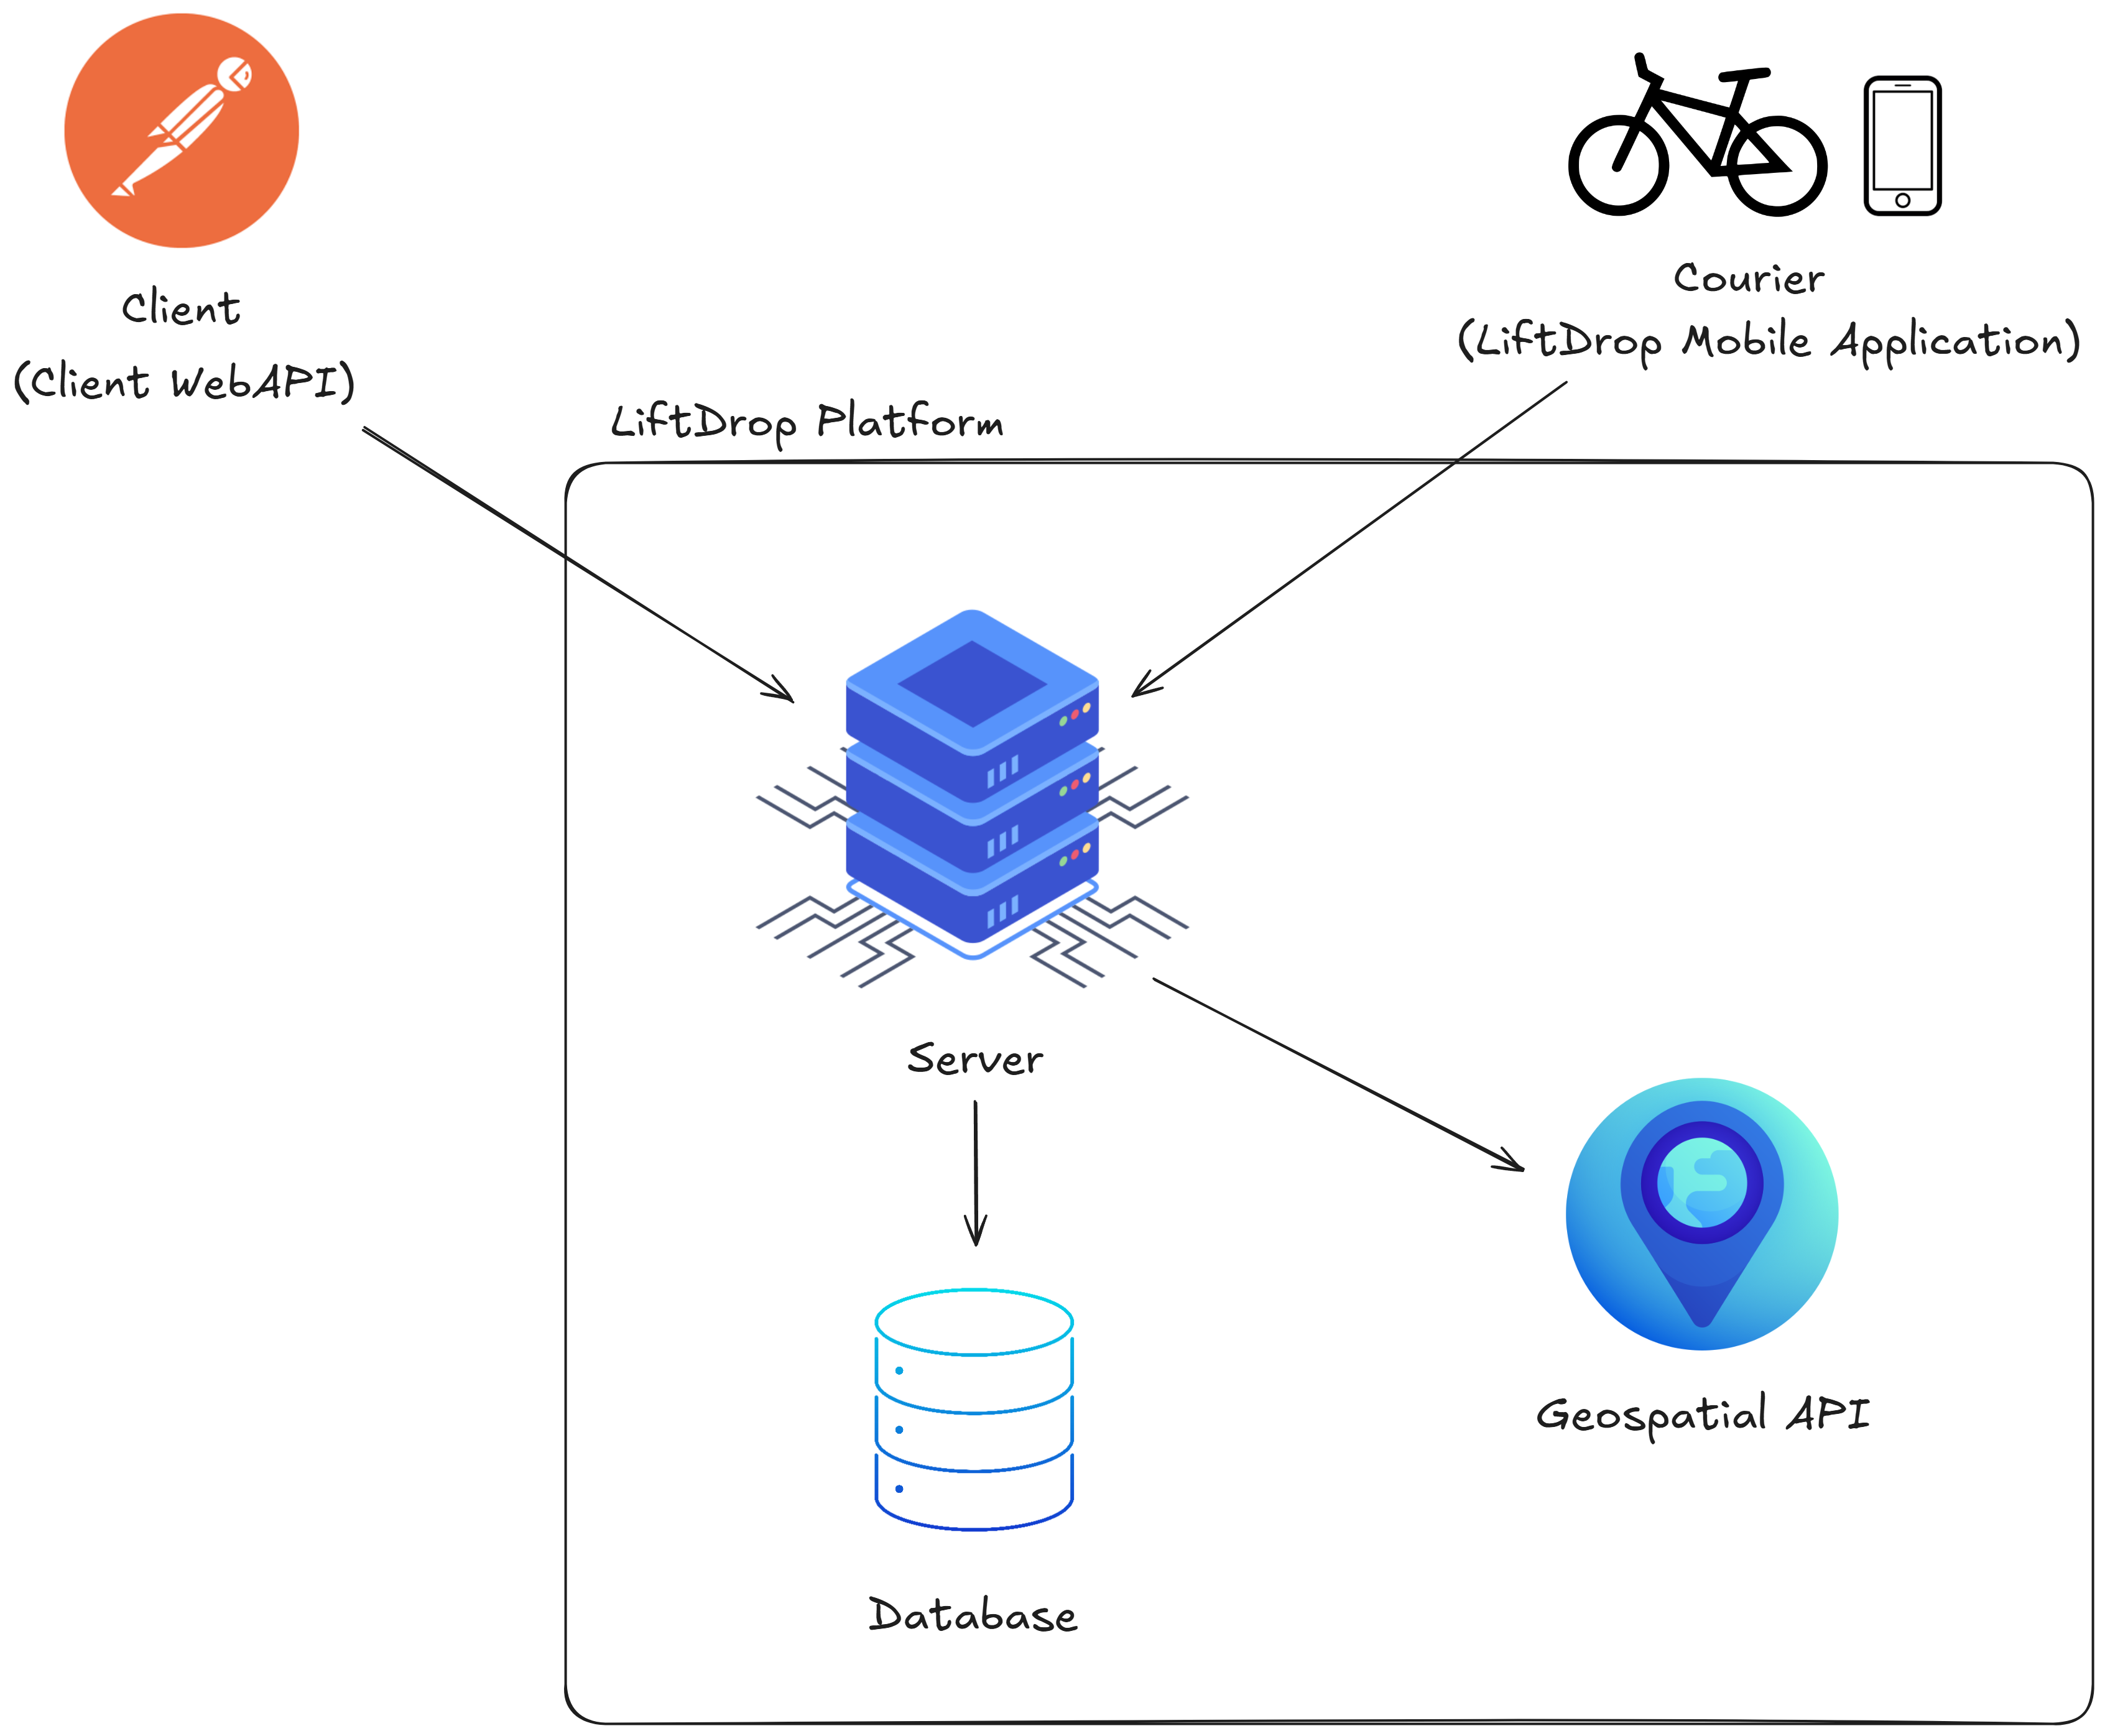
\includegraphics[width=0.8\textwidth]{images/LiftDrop_High_level_view.png}
    \caption{High-level overview of the platform, showing interaction between clients, server, database and external APIs (Google Maps).}
    \label{fig:high_level}
\end{figure}


\newpage

\section{Background and Project Scope}
\subsection{Background}

The rise of the gig economy has led to the widespread adoption of mobile platforms for urban logistics, enabling flexible, on-demand delivery through services like Uber Eats, Glovo, and Deliveo. These applications rely on real-time geolocation, cloud-based infrastructure, and efficient routing to connect couriers and clients in fast-paced environments.

In developing \textbf{LiftDrop}, we sought to build on these foundational ideas by prioritizing clarity, responsiveness, and user autonomy. Our goal is to design a system that supports couriers through timely communication, real-time updates, and context-aware feedback.

\vspace{2mm}

\subsection*{Technical Inspirations}

LiftDrop incorporates several key technologies and design principles:

\begin{itemize}
    \item Real-time geolocation and distance-based filtering via the Google Maps API
    \item Bidirectional communication between couriers and the server using WebSockets
    \item A modular backend architecture that supports role-based access for clients and couriers.
\end{itemize}

\vspace{2mm}

\subsection{Project Scope}

This section defines the functional and technical boundaries of the LiftDrop platform. It outlines the key features available to clients and couriers, the strategies for real-time data communication and order assignment. It also clarifies what the system is designed to accomplish and what lies outside the current scope of the project.

\subsection{Platform Features}

\subsubsection{Client Features}
\begin{itemize}
    \item Register with email, password, and address;
    \item Login with email and password;
    \item Add a drop-off point when placing an order;
    \item Place orders by selecting restaurants, items, and a drop-off point;
\end{itemize}

\subsubsection{Courier Features}
\begin{itemize}
    \item Register as a courier with name, email, and password;
    \item Login as a courier with email and password;
    \item Accept or decline delivery requests;
    \item Set availability by entering or exiting "listening" status;
    \item Cancel an accepted order;
    \item Confirm pickup with a code;
    \item Confirm delivery with a code upon completion;
\end{itemize}

\subsection{Real-Time Communication Strategy}

Real-time data communication is crucial for dynamic interactions and courier management. Three communication models were considered:

\begin{itemize}
    \item \textbf{Polling (Request-Response):} Simple but inefficient, causing excessive network overhead.
    \item \textbf{Server-Sent Events (SSE):} Effective for unidirectional updates, but limited in interaction complexity.
    \item \textbf{WebSockets:} Full-duplex communication that minimizes latency, ideal for bidirectional updates like order assignments, courier status changes, and live notifications.
\end{itemize}

\textbf{WebSockets} were chosen for their ability to support real-time, bidirectional communication, ensuring dynamic and efficient interaction between couriers and the system.

\subsection{Order Assignment Strategy}

Order assignments consider the following criteria to ensure efficiency:

\begin{itemize}
    \item \textbf{Proximity:} Couriers closest to the pickup location are prioritized.
    \item \textbf{Traffic Conditions:} Real-time traffic data helps optimize delivery time.
    \item \textbf{Courier Rating: } Courier Ratings are taken in consideration when choosing the order for which couriers receive orders.
\end{itemize}

The system integrates the \textbf{Google Maps API} for geospatial data, route optimization, and traffic-aware services to support efficient order assignment.

\subsection{User Roles}
The platform operates with distinct user roles:
\begin{itemize}
    \item \textbf{Clients:} Individuals who place orders for delivery. They can track their orders, add drop-off points, and receive updates on delivery status.
    \item \textbf{Couriers:} Individuals who fulfill delivery orders. They can accept or reject assignments, set availability, and confirm pickups and deliveries.
\end{itemize}


\section{System Design}

\subsection{User Journeys}

\subsubsection{Client Journey}

\bigskip

\begin{figure}[H]
    \centering
    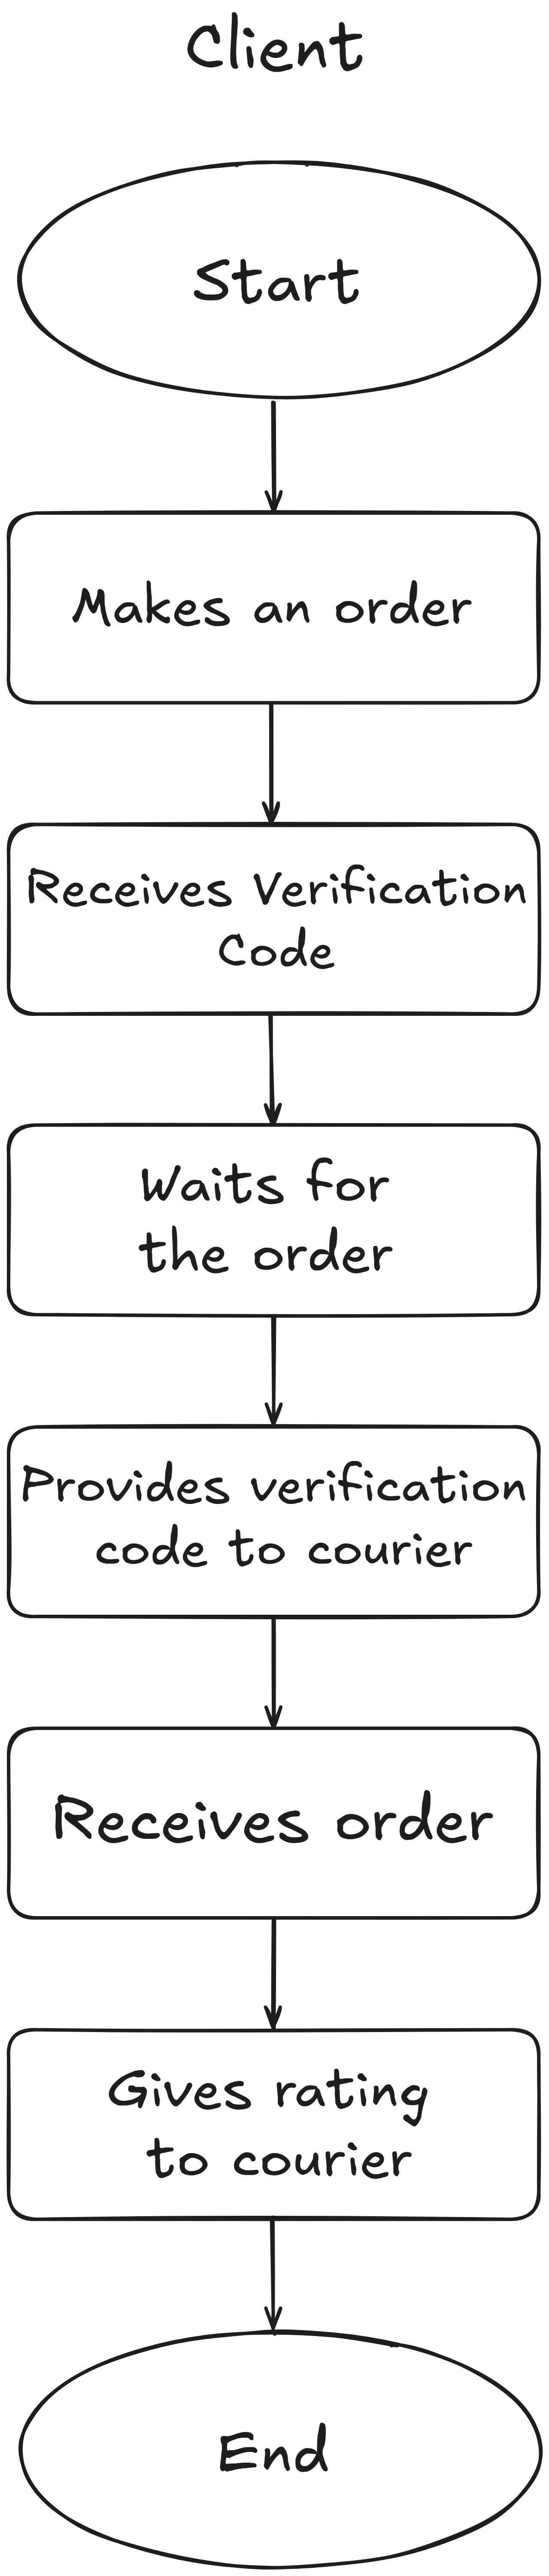
\includegraphics[width=0.2\textwidth]{images/ClientJourney.png} % adjust path & width if needed
    \caption{Client journey flowchart showing from the beginning}
    \label{fig:client_journey}
\end{figure}

This flowchart (\ref{fig:client_journey}) illustrates the sequential steps a client undergoes when placing an order through the LiftDrop platform. The process begins with the client initiating an order, followed by a waiting period for the order to be processed and accepted by a courier. Once the order is received, the client provides a unique confirmation code to the courier, marking a secure handoff. Finally, the process concludes with the client rating the delivery experience.

\newpage

\subsubsection{Courier Journey}

\bigskip

\begin{figure}[H]
    \centering
    \includegraphics[width=0.37\textwidth]{images/CourierJourney.png} % adjust path & width if needed
    \caption{Courier journey flowchart showing from the beginning}
    \label{fig:courier_journey}
\end{figure}

This flowchart (\ref{fig:courier_journey}) outlines the step-by-step decision-making process a courier follows while managing delivery requests on the LiftDrop platform. It begins with the courier awaiting an incoming order, which can either be accepted or rejected. Upon accepting a request, the courier proceeds to the pickup location, with the option to cancel if necessary. After pickup, the courier advances to the delivery phase. If the courier successfully reaches the destination, the delivery is confirmed. If the destination is not reached, the system prompts reevaluation or cancellation.

\newpage

\vspace{2mm}

\subsection{Interface Design}

The LiftDrop application includes distinct UI flows that guide couriers through each stage of the delivery lifecycle. This section presents key interface screens, organized by functionality and user context.

%\newpage

\subsubsection{Authentication Flow}

The authentication flow allows users to securely access the platform through account registration and login.

\begin{figure}[H]
    \centering
    \begin{subfigure}[b]{0.44\textwidth}
        \centering
        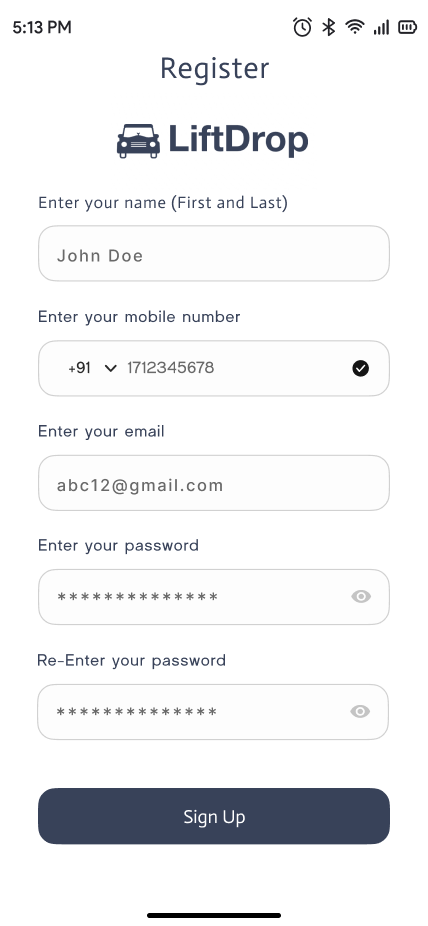
\includegraphics[width=\textwidth]{images/registration.png}
        \caption{User registration screen}
        \label{fig:registration}
    \end{subfigure}
    \hfill
    \begin{subfigure}[b]{0.44\textwidth}
        \centering
        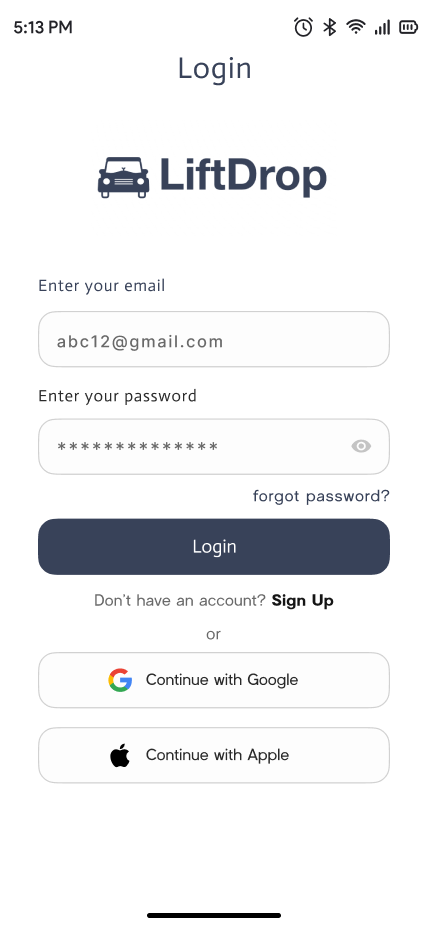
\includegraphics[width=\textwidth]{images/login.png}
        \caption{User login screen}
        \label{fig:login}
    \end{subfigure}
    \caption{Authentication flow screens in LiftDrop}
    \label{fig:auth_flow}
\end{figure}

\noindent\textbf{Registration Screen (\ref{fig:registration}):}  
Enables users to create an account by providing their name, email, and password.

\noindent\textbf{Login Screen (\ref{fig:login}):}  
Provides a simple interface for returning users to log in with their credentials.

\subsubsection{Courier Flow}

The following screens illustrate the courier experience—from going online to completing a delivery.

\begin{figure}[H]
    \centering
    \begin{subfigure}[b]{0.48\textwidth}
        \centering
        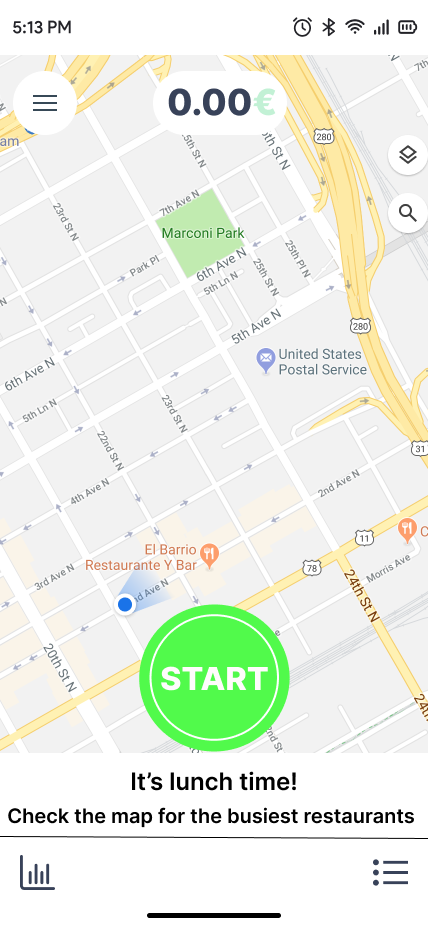
\includegraphics[width=\textwidth]{images/go_screen.png}
        \caption{Idle status screen}
        \label{fig:go_screen}
    \end{subfigure}
    \hfill
    \begin{subfigure}[b]{0.48\textwidth}
        \centering
        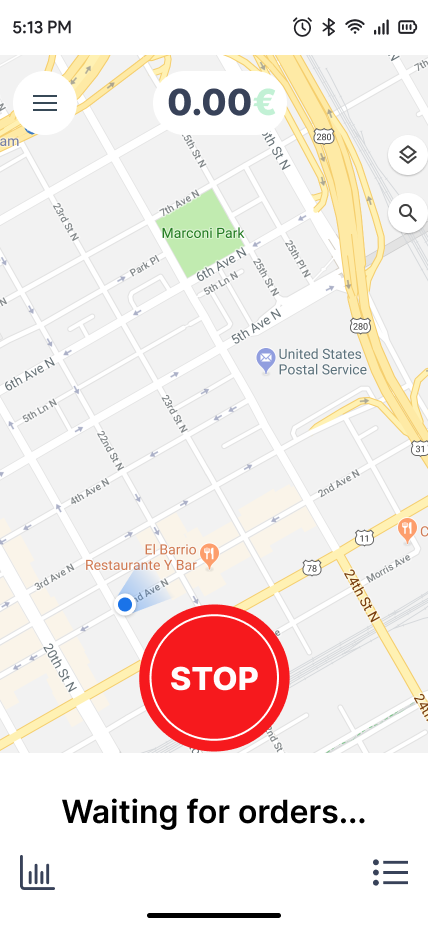
\includegraphics[width=\textwidth]{images/waiting_screen.png}
        \caption{Waiting for order screen}
        \label{fig:waiting_screen}
    \end{subfigure}
    \caption{Courier status screens during online session}
    \label{fig:courier_status}
\end{figure}

\noindent\textbf{Idle Screen (\ref{fig:go_screen}):}  
Allows couriers to toggle availability and begin accepting orders.

\noindent\textbf{Waiting Screen (\ref{fig:waiting_screen}):}  
Indicates that the system is searching for nearby orders in real time.

\begin{figure}[H]
    \centering
    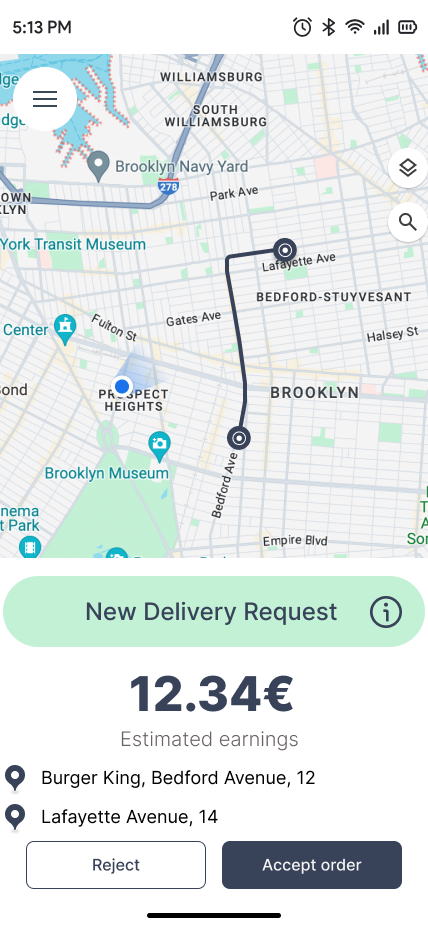
\includegraphics[width=0.6\textwidth]{images/delivery_request.png}
    \caption{Incoming delivery request with order summary and action buttons}
    \label{fig:delivery_request}
\end{figure}

\noindent\textbf{Delivery Request (\ref{fig:delivery_request}):}  
Displays order metadata such as pickup and drop-off addresses, delivery distance, and quick actions to accept or decline.

\begin{figure}[H]
    \centering
    \begin{subfigure}[b]{0.48\textwidth}
        \centering
        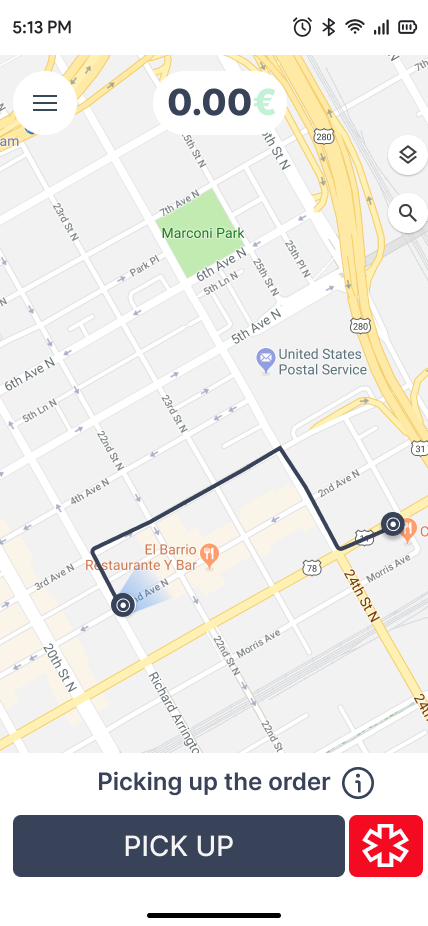
\includegraphics[width=\textwidth]{images/pickup_order_screen.png}
        \caption{Pickup confirmation screen}
        \label{fig:pickup_order}
    \end{subfigure}
    \hfill
    \begin{subfigure}[b]{0.48\textwidth}
        \centering
        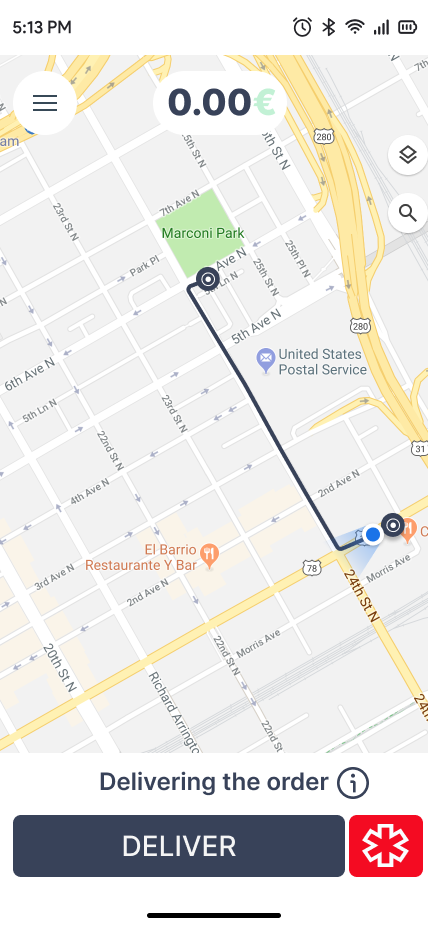
\includegraphics[width=\textwidth]{images/deliver_order_screen.png}
        \caption{Delivery confirmation screen}
        \label{fig:deliver_order}
    \end{subfigure}
    \caption{Screens for confirming pickup and delivery}
    \label{fig:courier_pickup_deliver}
\end{figure}

\noindent\textbf{Pickup Screen (\ref{fig:pickup_order}):}  
Guides the courier to confirm pickup, with cancelation support and verification of PIN.

\noindent\textbf{Delivery Screen (\ref{fig:deliver_order}):}  
Guides the courier to confirm delivery, with cancelation support and verification of PIN.

\newpage

\subsection{System Architecture and Data Model}

This section presents different architectural perspectives of the LiftDrop system, including component-level interactions and data model relationships. Each view emphasizes a specific aspect of the system's behavior, from geolocation handling to user roles and delivery lifecycle.

\subsubsection{High-Level System Architecture}

Figure~\ref{fig:high-level-Overview} illustrates the top-level architecture of the LiftDrop platform. It shows how the Android mobile application communicates with backend services responsible for order management, user interaction, real-time communication, and location processing.

\vspace{8mm}

\begin{figure}[H]
    \centering
    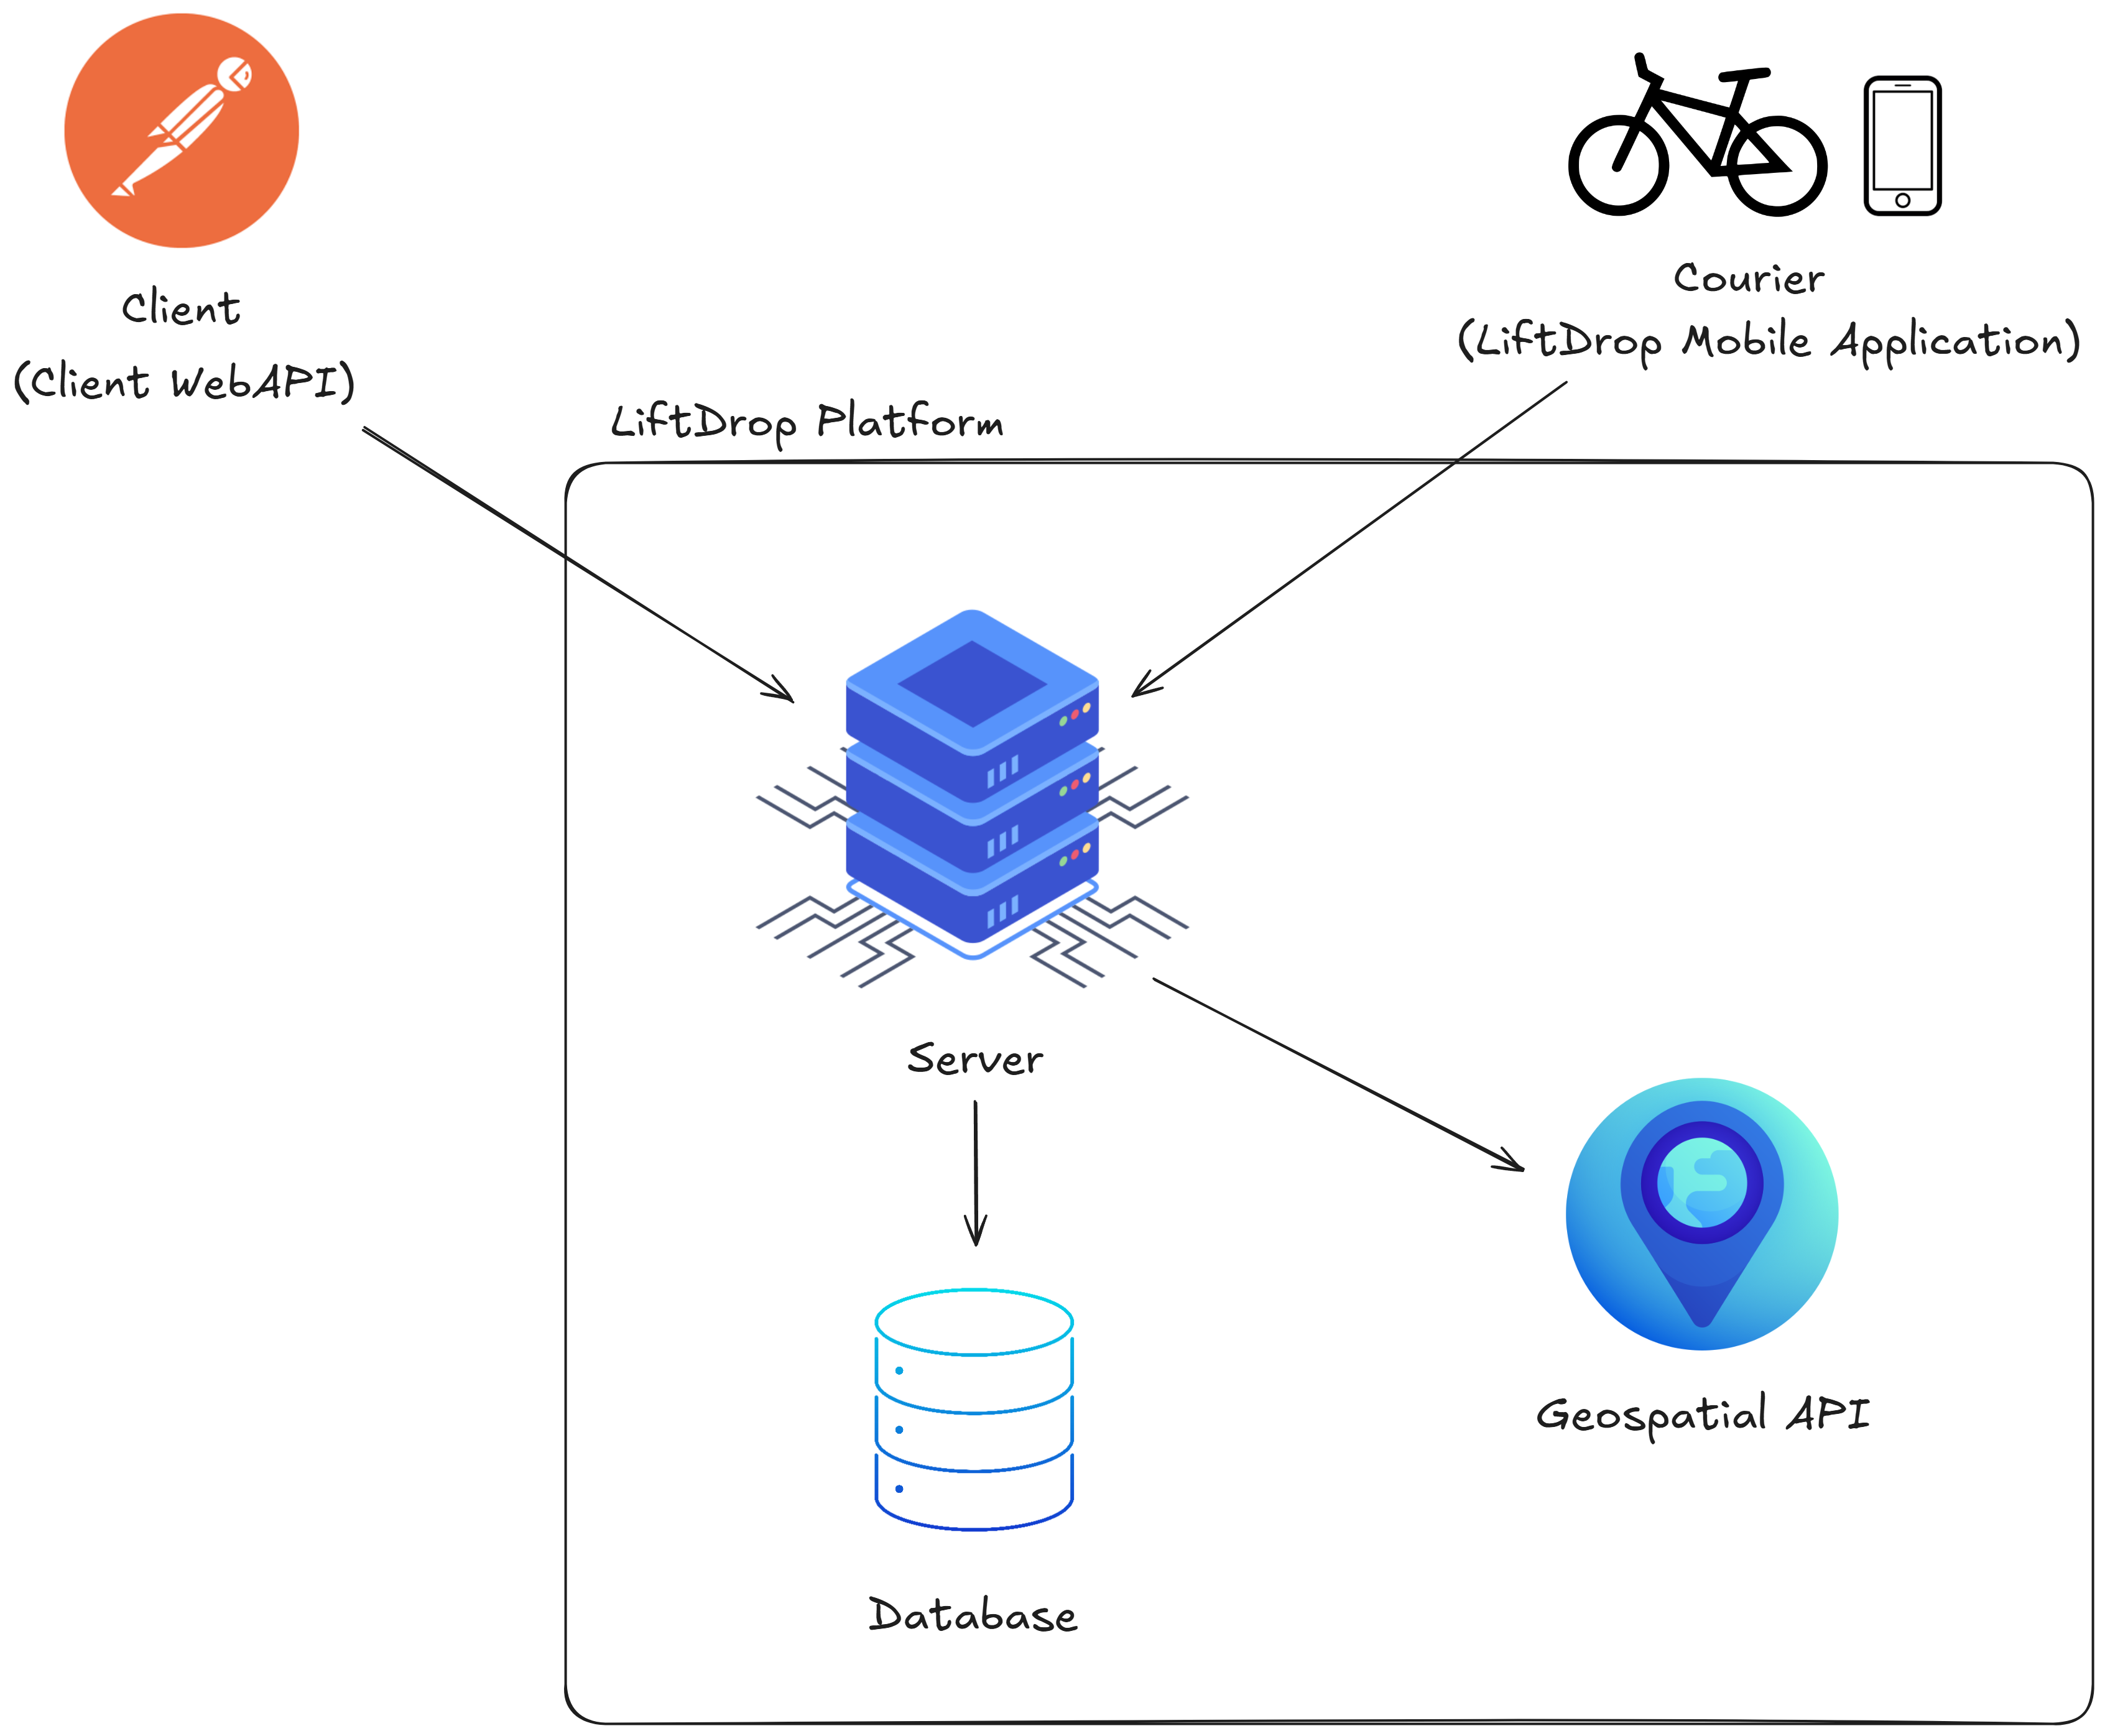
\includegraphics[width=0.82\textwidth]{images/LiftDrop_High_level_view.png}
    \caption{High-level overview of the LiftDrop system architecture}
    \label{fig:high-level-Overview}
\end{figure}

\newpage

\subsubsection{Location Model Overview}

This view isolates the system's handling of geospatial information. The \texttt{Location} class acts as a base abstraction for different types of spots used during a delivery. Specialized entities like \texttt{PickupSpot} and \texttt{DropOffSpot} inherit from \texttt{Location}, allowing consistent treatment of position data. A pickup spot can contain multiple \texttt{Item} entries, each identified by a unique designation.

\begin{figure}[H]
    \centering
    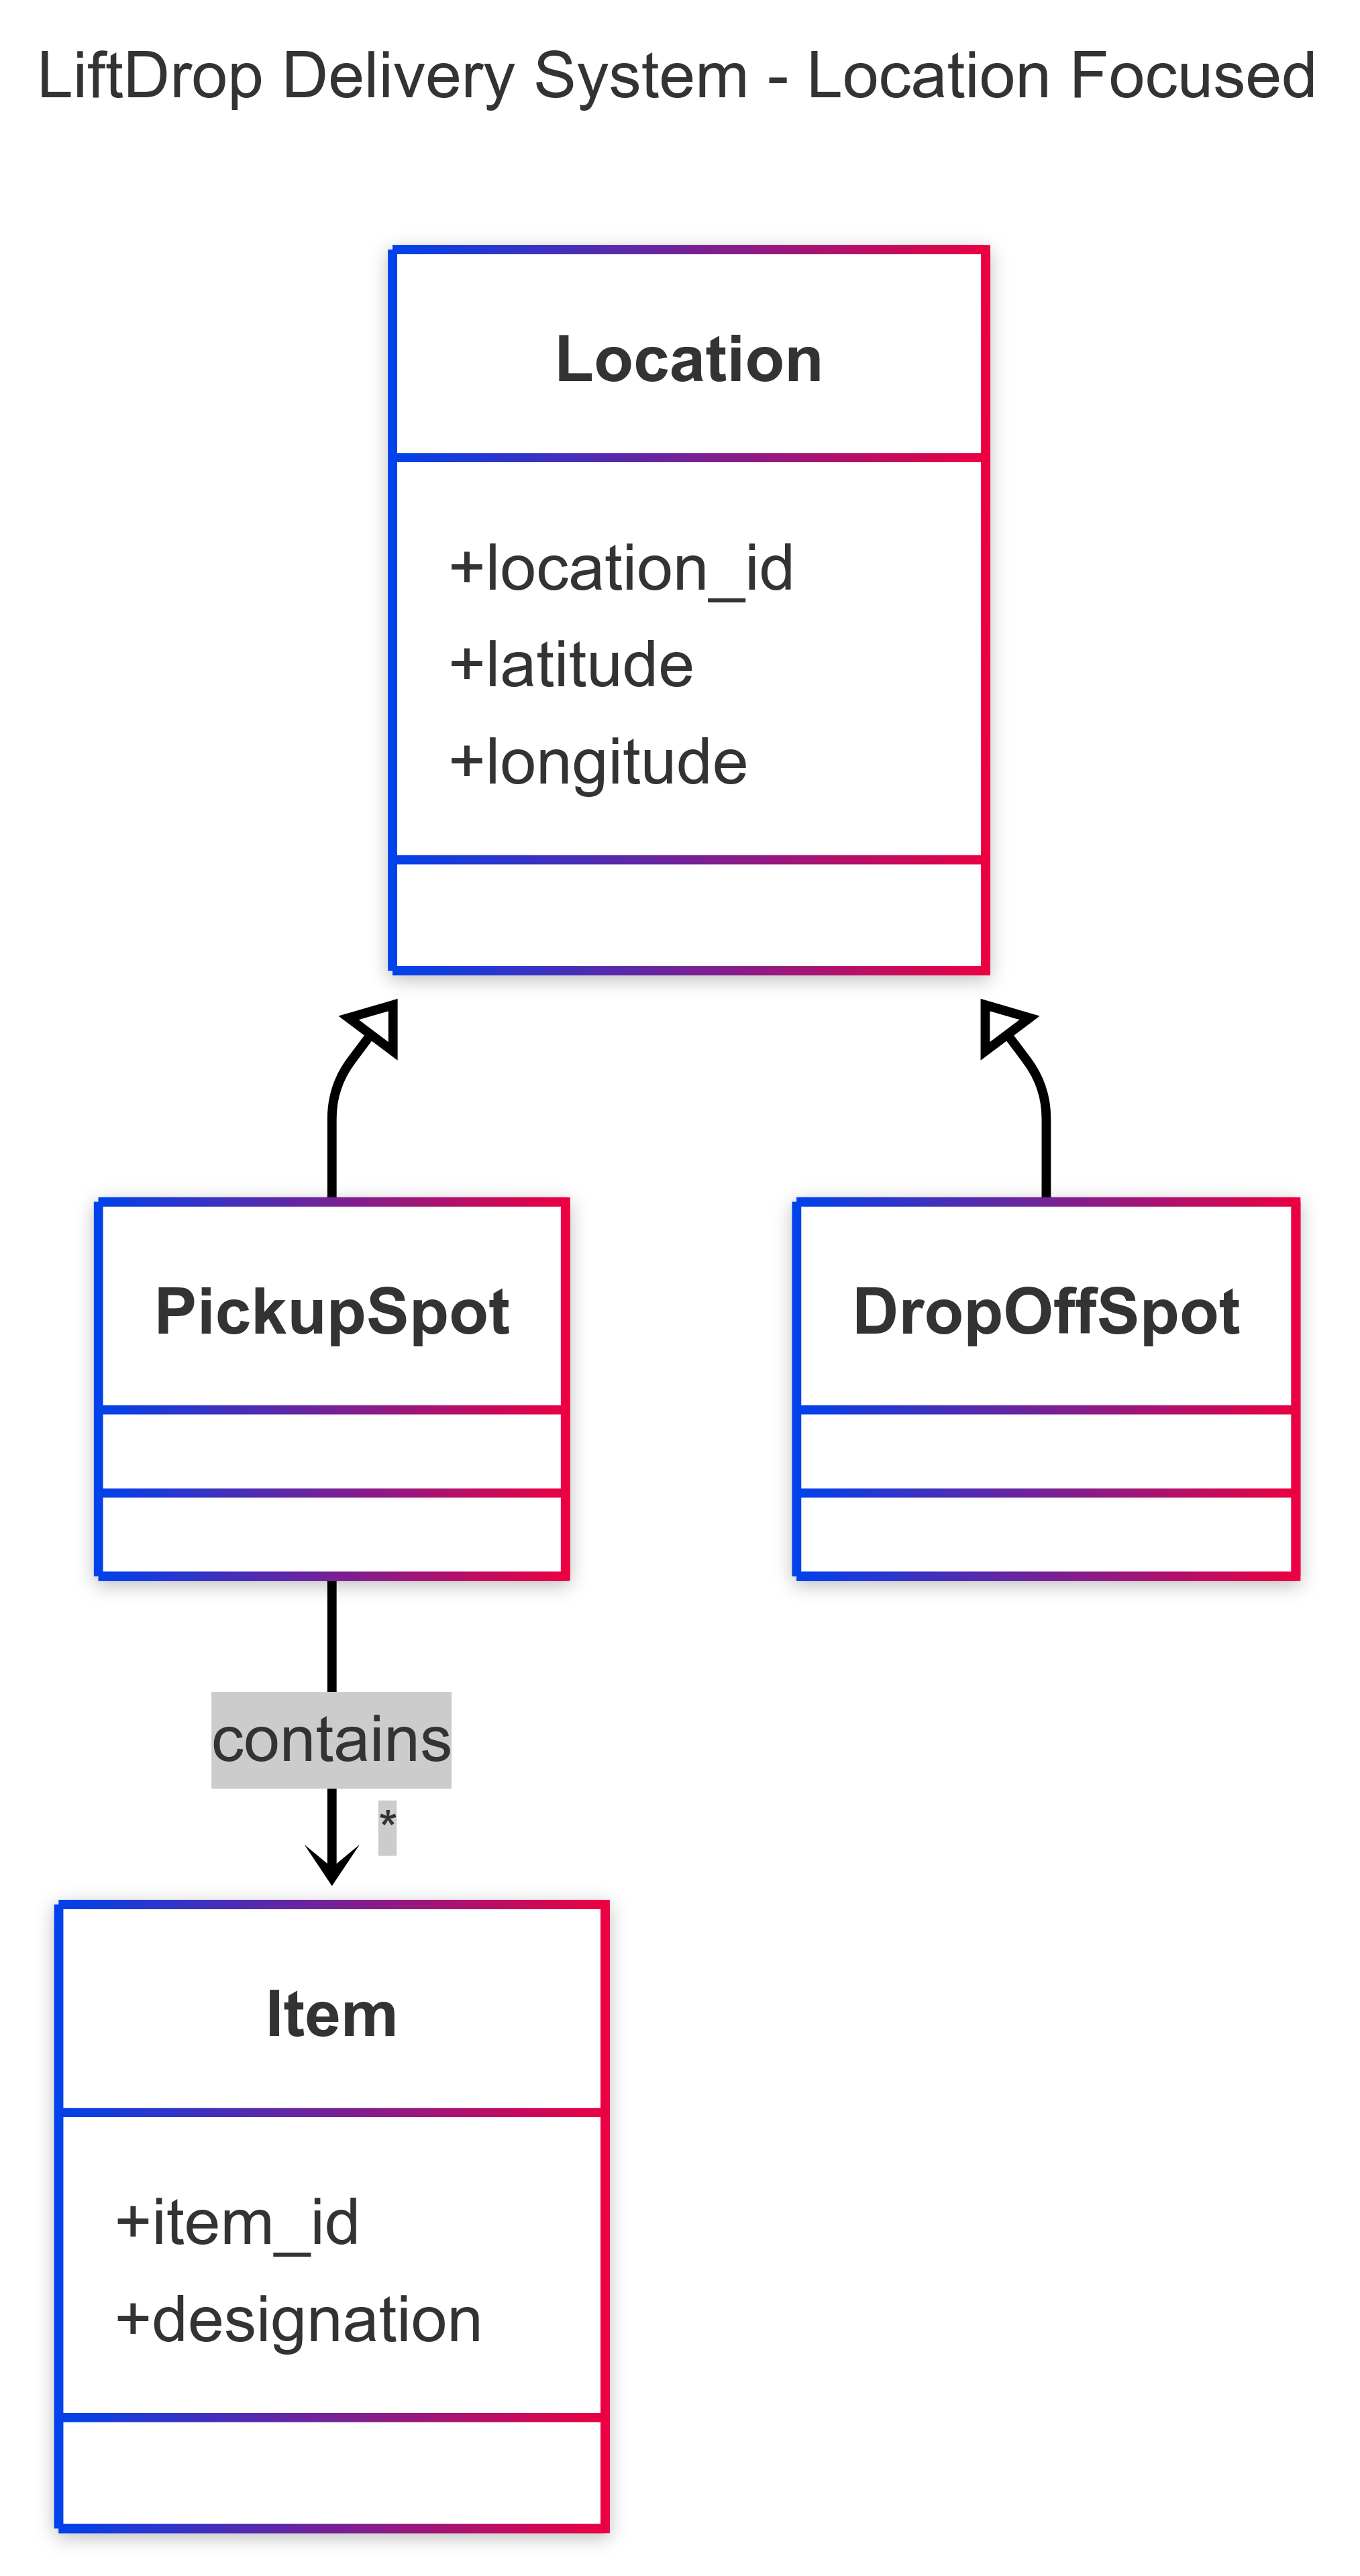
\includegraphics[width=0.44\textwidth]{images/LocationDiagram.png}
    \caption{Location Model Structure}
\end{figure}

\newpage

\subsubsection{User Role and Interaction Model}

This simplified diagram captures user roles and their interaction with delivery workflows. A \texttt{Client} can place multiple \texttt{Request}s, and a \texttt{Courier} can fulfill many of them. Each request is linked to a corresponding \texttt{Delivery}, forming a one-to-one mapping between a request and its fulfillment.
  
\begin{figure}[H]
    \centering
    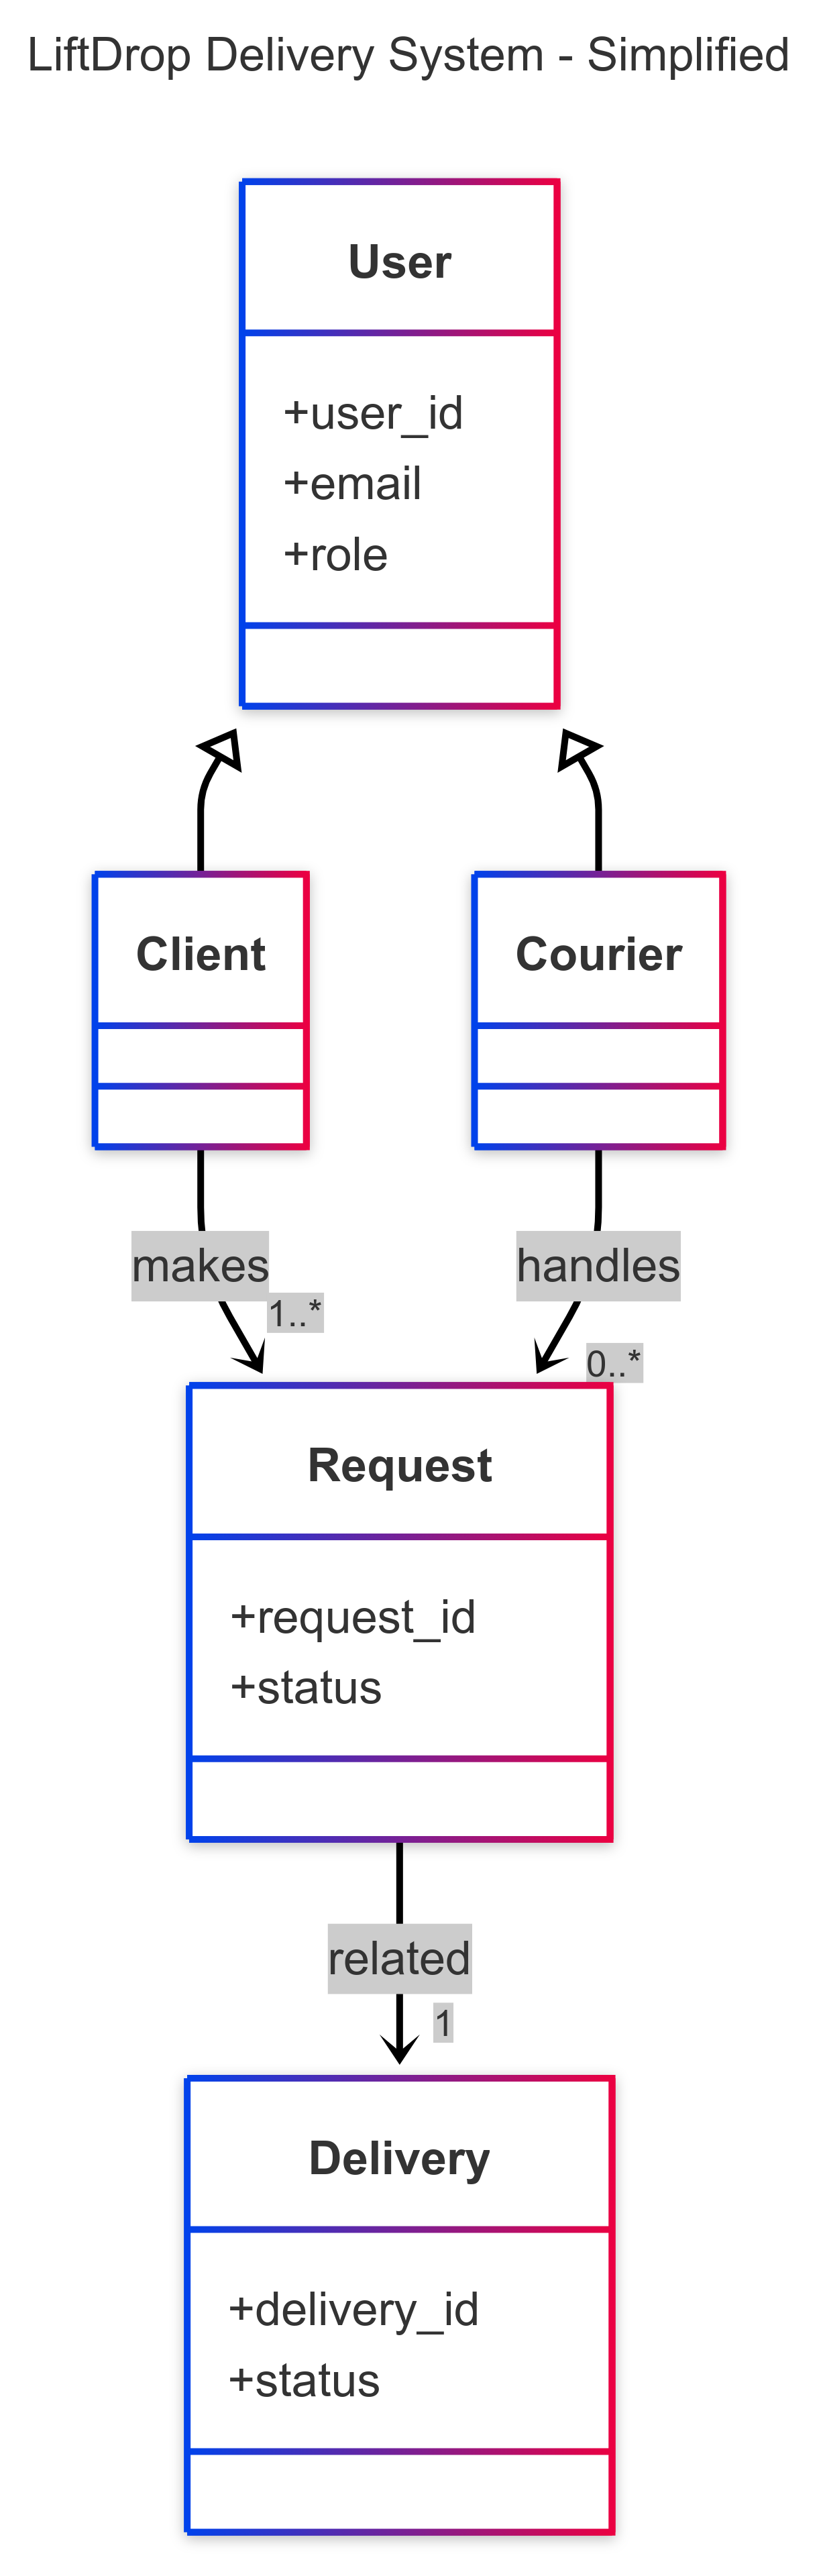
\includegraphics[width=0.40\textwidth]{images/UserClientCourierDiagram.png}
    \caption{User and Role Relationships}
\end{figure}

\subsubsection{Request and Delivery Lifecycle View}

This view focuses on how a request progresses through the system. Each \texttt{Request} includes additional metadata encapsulated in a \texttt{RequestDetails} object and is associated with a single \texttt{Delivery}. This structure supports clear traceability and separation of concerns between request creation and execution.

\begin{figure}[H]
    \centering
    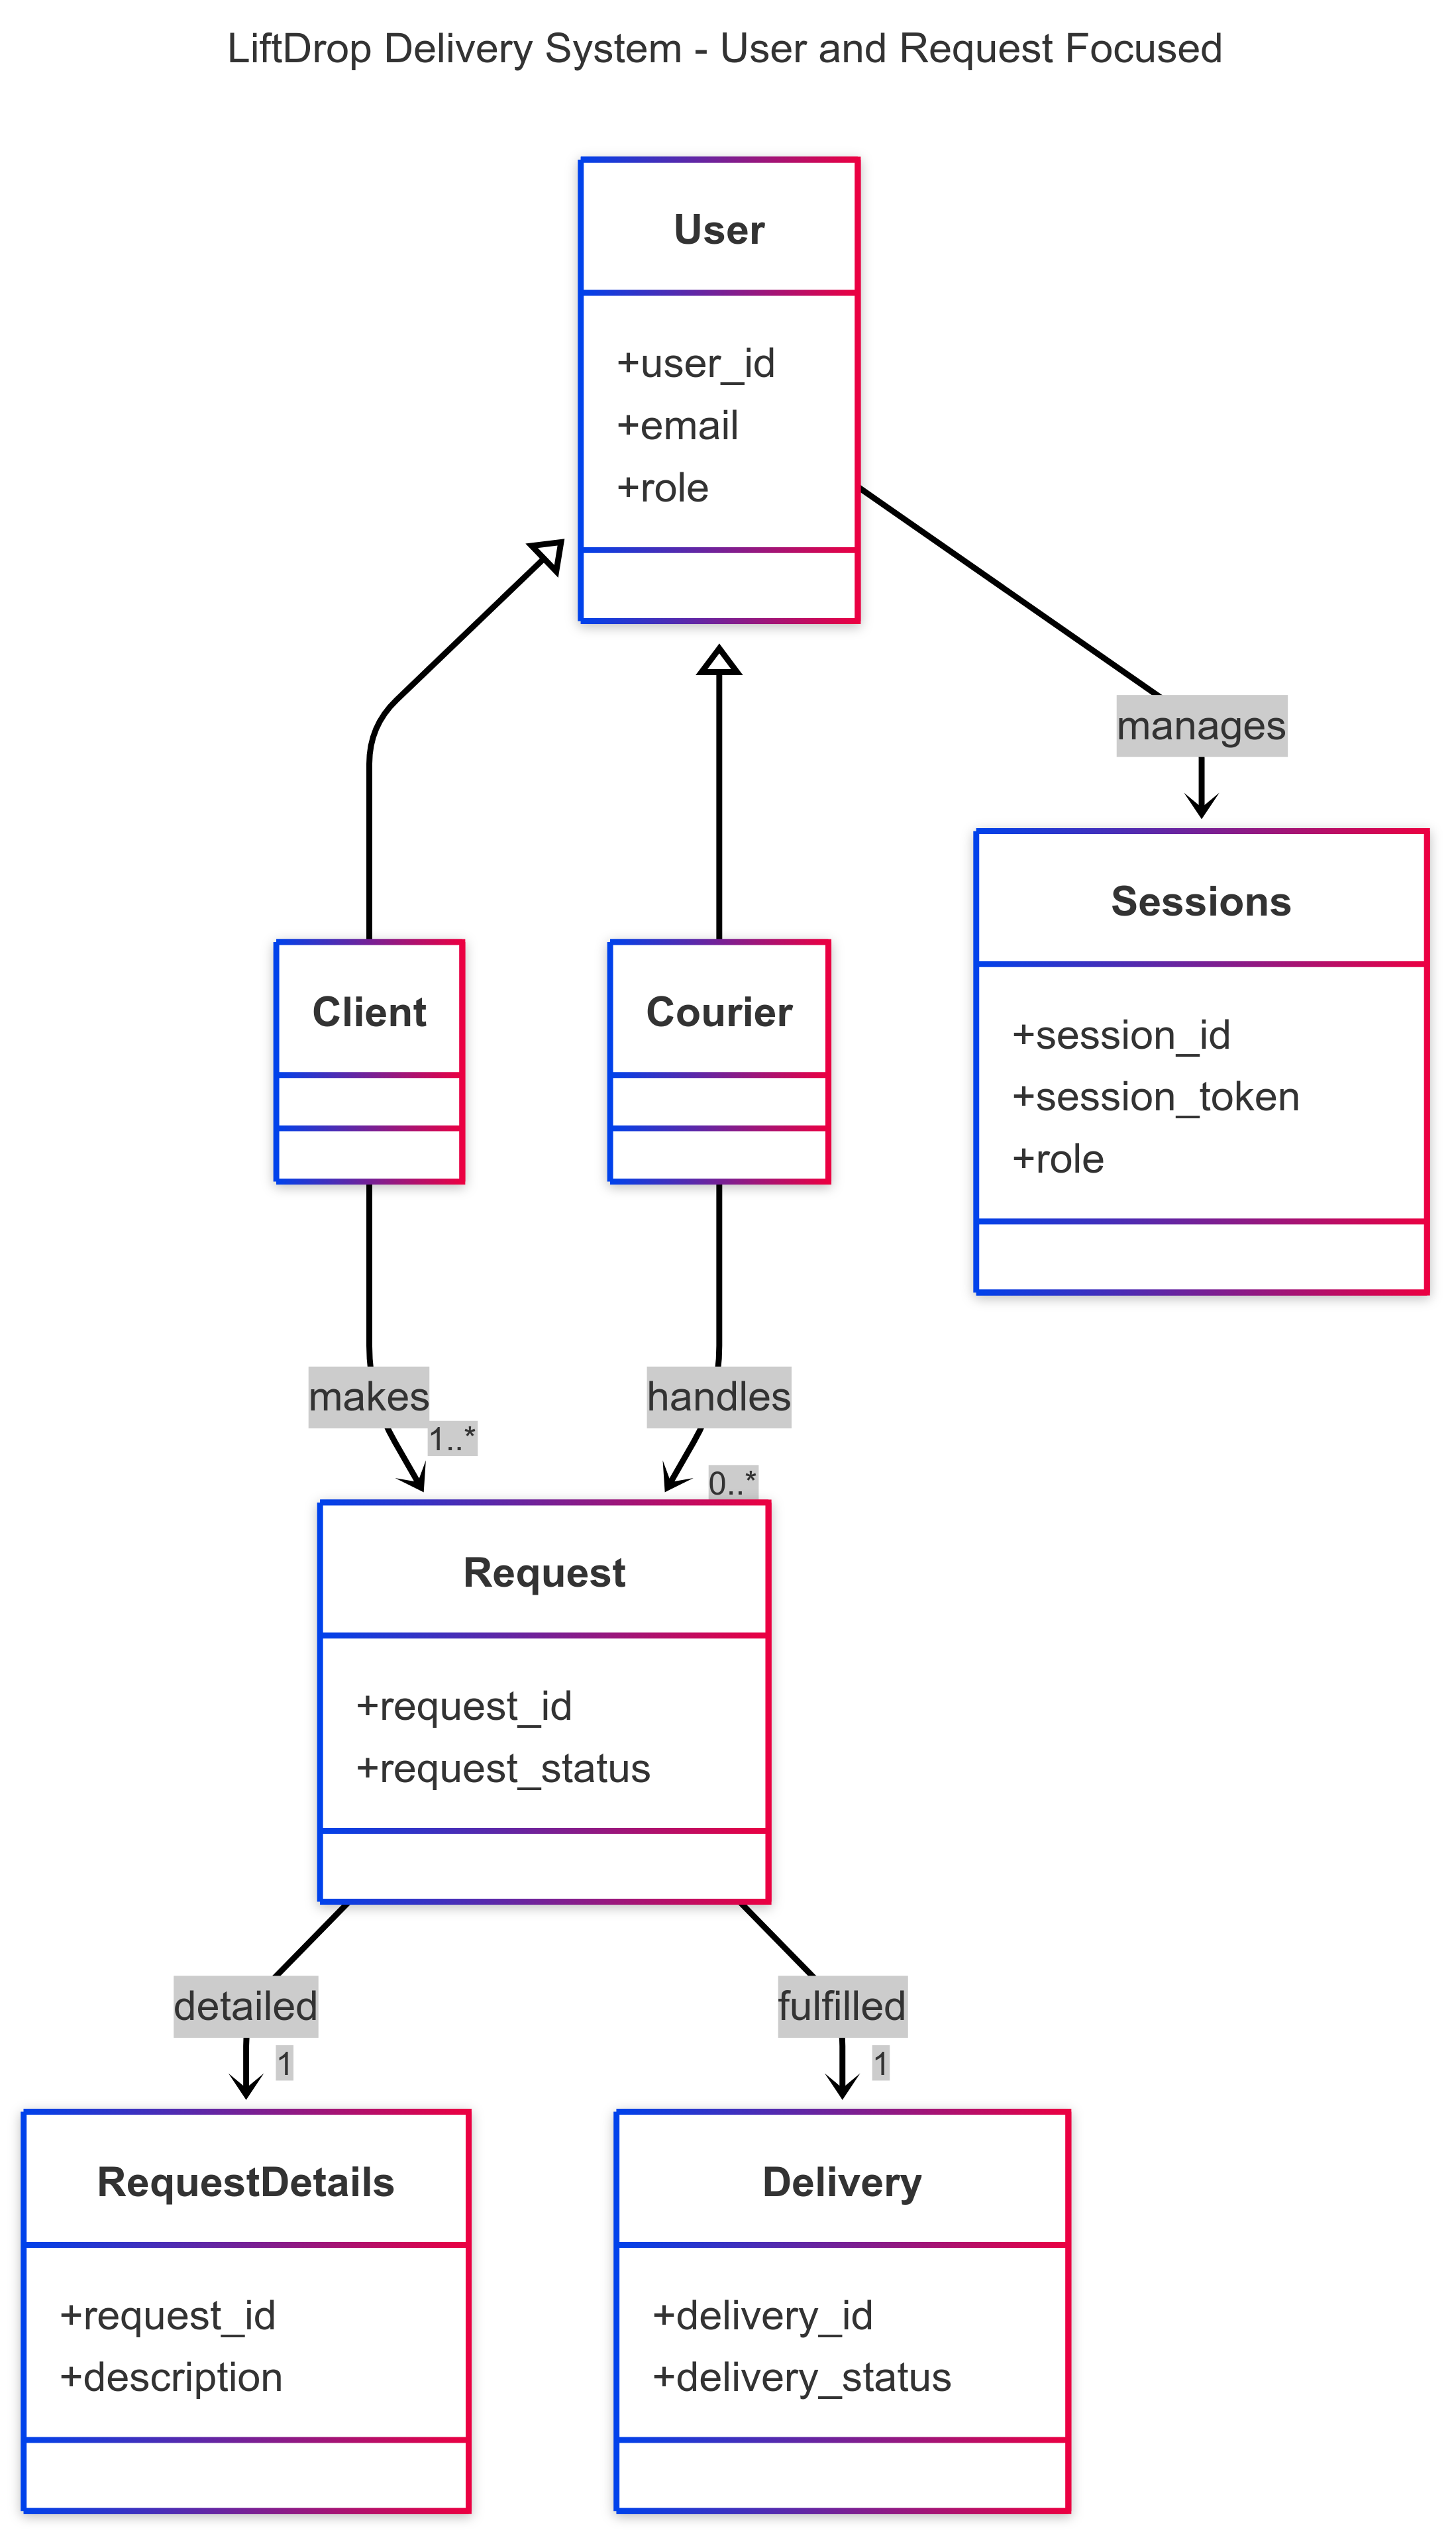
\includegraphics[width=0.44\textwidth]{images/UserSessions.png}
    \caption{Request and Fulfillment Architecture}
\end{figure}

\newpage

\subsubsection{Comprehensive System Model}

The complete data model integrates all key domain entities: \texttt{User}, \texttt{Address}, \texttt{Location}, \texttt{Item}, \texttt{Request}, \texttt{Delivery}, and \texttt{Session}. It captures how users interact with the system, how orders are structured and routed, and how real-time delivery coordination is maintained through geolocation and session-aware tracking.

\begin{figure}[H]
    \centering
    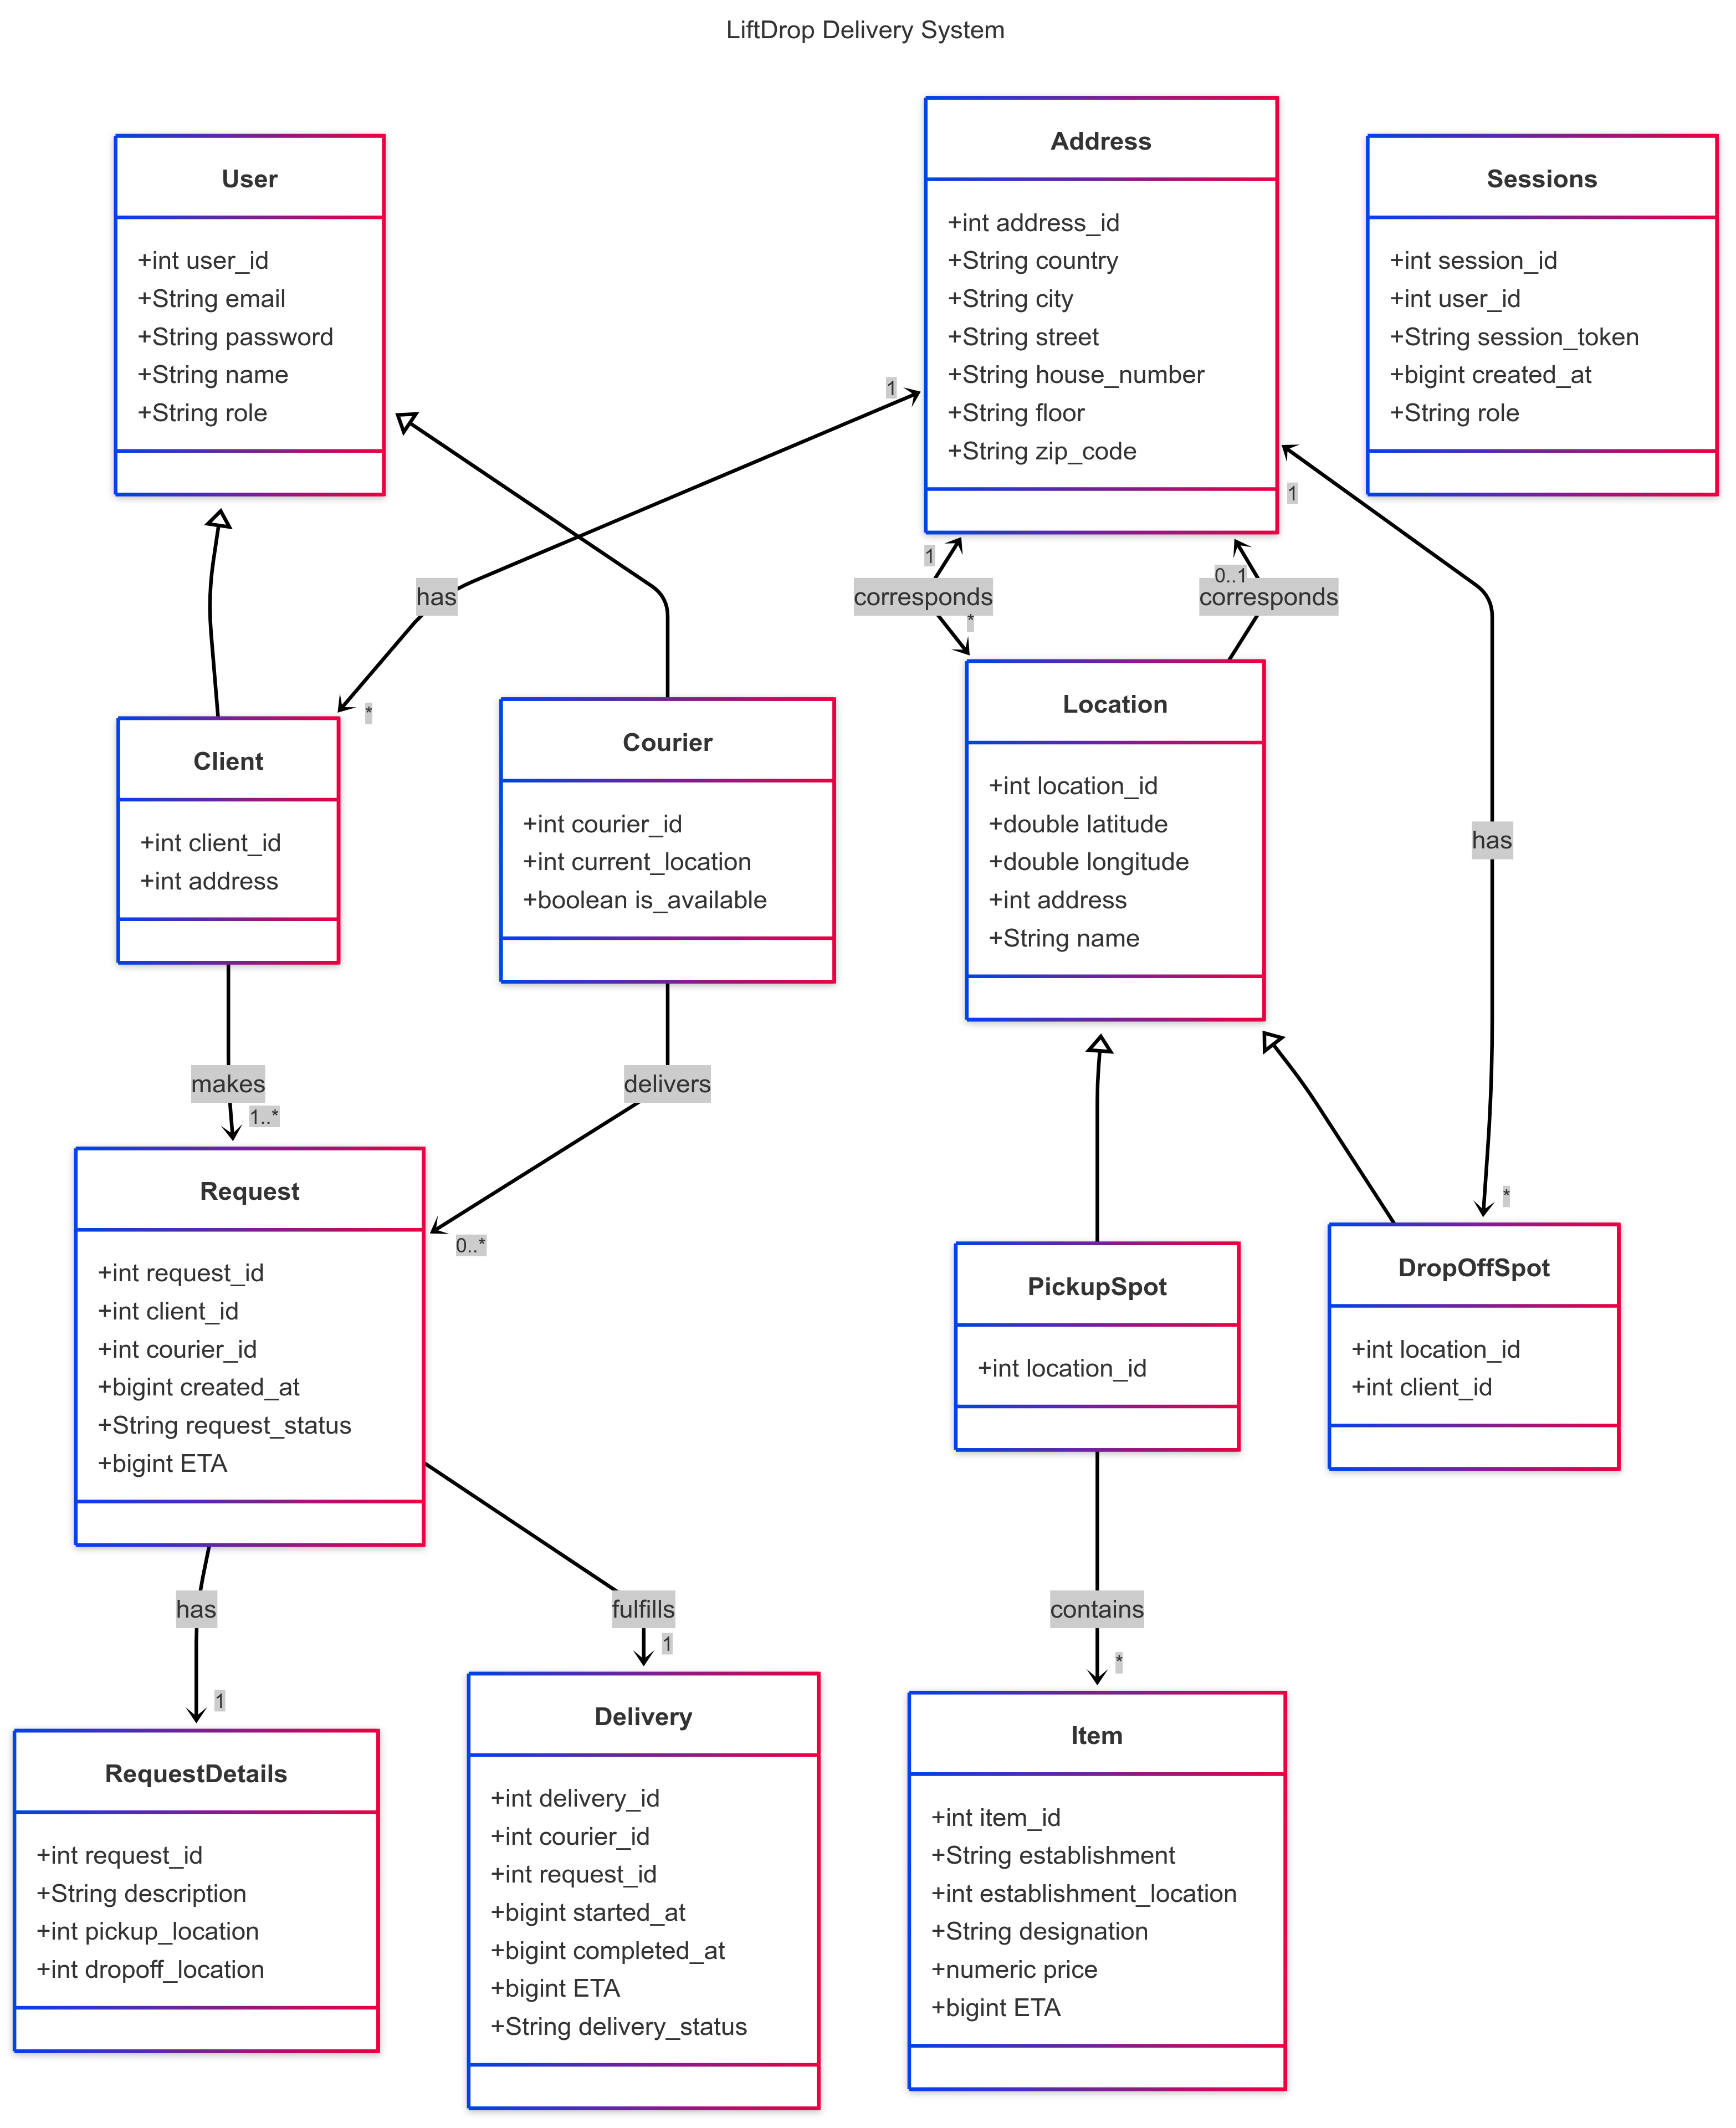
\includegraphics[width=0.8\textwidth]{images/FullDiagram.png}
    \caption{Full System Data Model}
\end{figure}



\section{Technical Implementation Details}

This section outlines the core technologies and tools employed in the development of the LiftDrop platform, along with key decisions regarding communication, backend logic, and security.

\subsection{Technology Stack}
\begin{itemize}
    \item \textbf{Mobile Application}: Developed using Android Jetpack Compose (Kotlin), the app enables couriers to manage order availability, accept or reject requests, and track deliveries in real time.
    \item \textbf{Backend Server}: Built with Spring Web MVC, the server handles business logic, order assignment, and serves API endpoints for communication with the mobile application.
    \item \textbf{Database}: PostgreSQL is utilized for the structured storage of essential data, including user profiles, orders, delivery statuses, and location history.
    \item \textbf{Geospatial Services}: The Google Maps API is leveraged for calculating courier distances, estimating delivery times, and optimizing routes based on live traffic conditions.
\end{itemize}

\subsection{Communication Protocol}

To facilitate real-time updates between the mobile application and the backend server, \textbf{WebSockets} are used. WebSockets offer several advantages over alternatives like polling and Server-Sent Events (SSE), including bidirectional communication, reduced latency, and minimized network overhead. These benefits ensure a more responsive and interactive experience for couriers, particularly when managing order updates and status changes.

The courier's location is continuously updated using \textbf{Foreground Services} on Android. This approach ensures the app maintains an active connection, delivering real-time location data even when running in the background, and avoids being terminated by the operating system.

\subsection{Order Assignment Logic}

Orders are assigned based on the following factors:
\begin{itemize}
    \item \textbf{Proximity to the pickup point}
    \item \textbf{Fair workload distribution} considering the courier’s recent delivery history
    \item \textbf{Live traffic conditions}, using geospatial data to optimize routing
\end{itemize}

\subsection{Security and Authentication}

To ensure secure user sessions and API requests:
\begin{itemize}
    \item \textbf{Session-Based Authentication with Cookies}: After a successful login, the server sets an HTTP-only cookie containing a session token. This token is inaccessible to JavaScript, which helps mitigate cross-site scripting (XSS) attacks.
\end{itemize}

\subsection{Development Tools}

\begin{itemize}
    \item \textbf{Postman}: Used to test and validate REST API endpoints during backend development.
    \item \textbf{Git and GitHub}: Employed for version control, collaboration, and managing the development workflow.
    \item \textbf{Android Studio}: The primary IDE for building, testing, and debugging the mobile courier application.
    \item \textbf{Intellij}: The primary IDE for building, testing, and debugging the backend.
\end{itemize}

\subsection{Deployment Details}

\begin{itemize}
    \item \textbf{Backend Deployment}: The backend is hosted on Render, a cloud platform that streamlines deployment and scaling processes.
    \item \textbf{Database Hosting}: PostgreSQL is managed and hosted on Render, providing a scalable, reliable environment for data storage.
\end{itemize}


\section{Limitations and Future Work}

While LiftDrop delivers a functional prototype focused on real-time delivery coordination and transparent courier interaction, several ideas and features were considered but not implemented due to time constraints or project scope boundaries.

\subsection{Unimplemented Features}

\begin{itemize}
    \item \textbf{Client Application Interface}: The current system includes a simulated client API for testing, but no dedicated client-facing mobile application was developed.
    
    \item \textbf{Administrative Dashboard}: A management panel for monitoring orders and courier activity.
    
    \item \textbf{Push Notifications}: All real-time updates currently rely on WebSockets; platform-native push notifications could enhance user engagement and reliability.

    \item \textbf{WebSocket Reconnection Support}: The WebSocket implementation currently lacks fault-tolerance mechanisms for automatic reconnection in case of network disruptions. This may affect delivery request communication stability on unreliable connections.
    
    \item \textbf{Courier Wait Time Compensation}: The current earnings model does not factor in courier wait time at pickup locations. Including this would ensure fairer compensation for delays caused by clients or merchants.
\end{itemize}

\subsection{Future Improvements}

\begin{itemize}
    \item \textbf{Internationalization (i18n)}: Support for multiple languages to make the app more inclusive for international users.

    \item \textbf{Resilient Real-Time Communication}: Replace or enhance WebSocket infrastructure with support for automatic reconnection and state synchronization to improve robustness in unstable network environments.

    \item \textbf{Enhanced Earnings Model}: Extend the current earnings calculation to include compensation for time spent waiting at pickup locations, in addition to distance and item value.

    \item \textbf{Courier Performance Analytics}: Introduce metrics for tracking delivery efficiency, response times, and reliability.
    
    \item \textbf{Scalability Testing}: The platform could benefit from stress testing under simulated high-traffic scenarios to identify performance bottlenecks.
\end{itemize}

This list reflects the balance between development priorities and available resources and serves as a guide for future iterations of the LiftDrop platform.


\section{Conclusion}

The development of the LiftDrop platform offered a practical exploration of the challenges involved in building real-time, location-aware delivery systems. Through the design and implementation of a courier-focused mobile application and supporting backend infrastructure, we aimed to simulate core components of modern gig economy services in a simplified but functional form.

Key aspects such as real-time communication via WebSockets, distance-based order assignment, and session-based authentication were successfully integrated and tested. Additionally, the modular architecture and transaction-safe database access layers provide a strong foundation for future enhancements and scalability.

Beyond technical implementation, this project allowed us to engage with broader questions around user experience, fairness, and system transparency. Although we chose not to implement features such as fairness algorithms or complex routing logic, the decisions we made were informed by both practical constraints and real-world platform behavior.

Ultimately, LiftDrop stands as a focused, extensible prototype that reflects our ability to apply software engineering principles, explore unfamiliar technologies, and reason through architectural trade-offs. Future work could expand the platform’s capabilities with client-facing applications, analytics, and more sophisticated operational tools.


%%%%%%%%%%%%%%%%
%%Bibliography%%
%%%%%%%%%%%%%%%%

\begin{thebibliography}{9}

\bibitem{spring}
Spring Framework. \textit{Spring Web MVC Documentation}. Available at: \url{https://spring.io/projects/spring-framework}

\bibitem{android}
Google Developers. \textit{Android Jetpack Compose}. Available at: \url{https://developer.android.com/jetpack/compose}

\bibitem{maps}
Google Cloud. \textit{Google Maps Platform Documentation}. Available at: \url{https://developers.google.com/maps/documentation}

\bibitem{postgres}
PostgreSQL Global Development Group. \textit{PostgreSQL Documentation}. Available at: \url{https://www.postgresql.org/docs/}

\bibitem{websockets}
MDN Web Docs. \textit{WebSockets}. Available at: \url{https://developer.mozilla.org/en-US/docs/Web/API/WebSocket}

\bibitem{jdbi}
JDBI Project. \textit{JDBI Documentation}. Available at: \url{https://jdbi.org/}

\bibitem{courierplatforms}
Glovo. \textit{How It Works for Couriers}. Available at: \url{https://glovoapp.com}

\bibitem{github}
GitHub Docs. \textit{Understanding the GitHub Flow}. Available at: \url{https://docs.github.com/en/get-started/quickstart/github-flow}

\bibitem{kotlin-docs}
JetBrains. \textit{Kotlin Language Documentation}. Available at: \url{https://kotlinlang.org/docs/home.html}. 

\bibitem{android-datastore}
Google. \textit{Jetpack DataStore}. Available at: \url{https://developer.android.com/topic/libraries/architecture/datastore}.

\bibitem{compose-state}
Google. \textit{State in Jetpack Compose}. Available at: \url{https://developer.android.com/jetpack/compose/state}.

\end{thebibliography}

% -------------------
% Blank Page
% -------------------
\newpage
\thispagestyle{empty}
\null
\newpage

\appendix

\section{EA Model}

\begin{figure}[H]
    \centering
    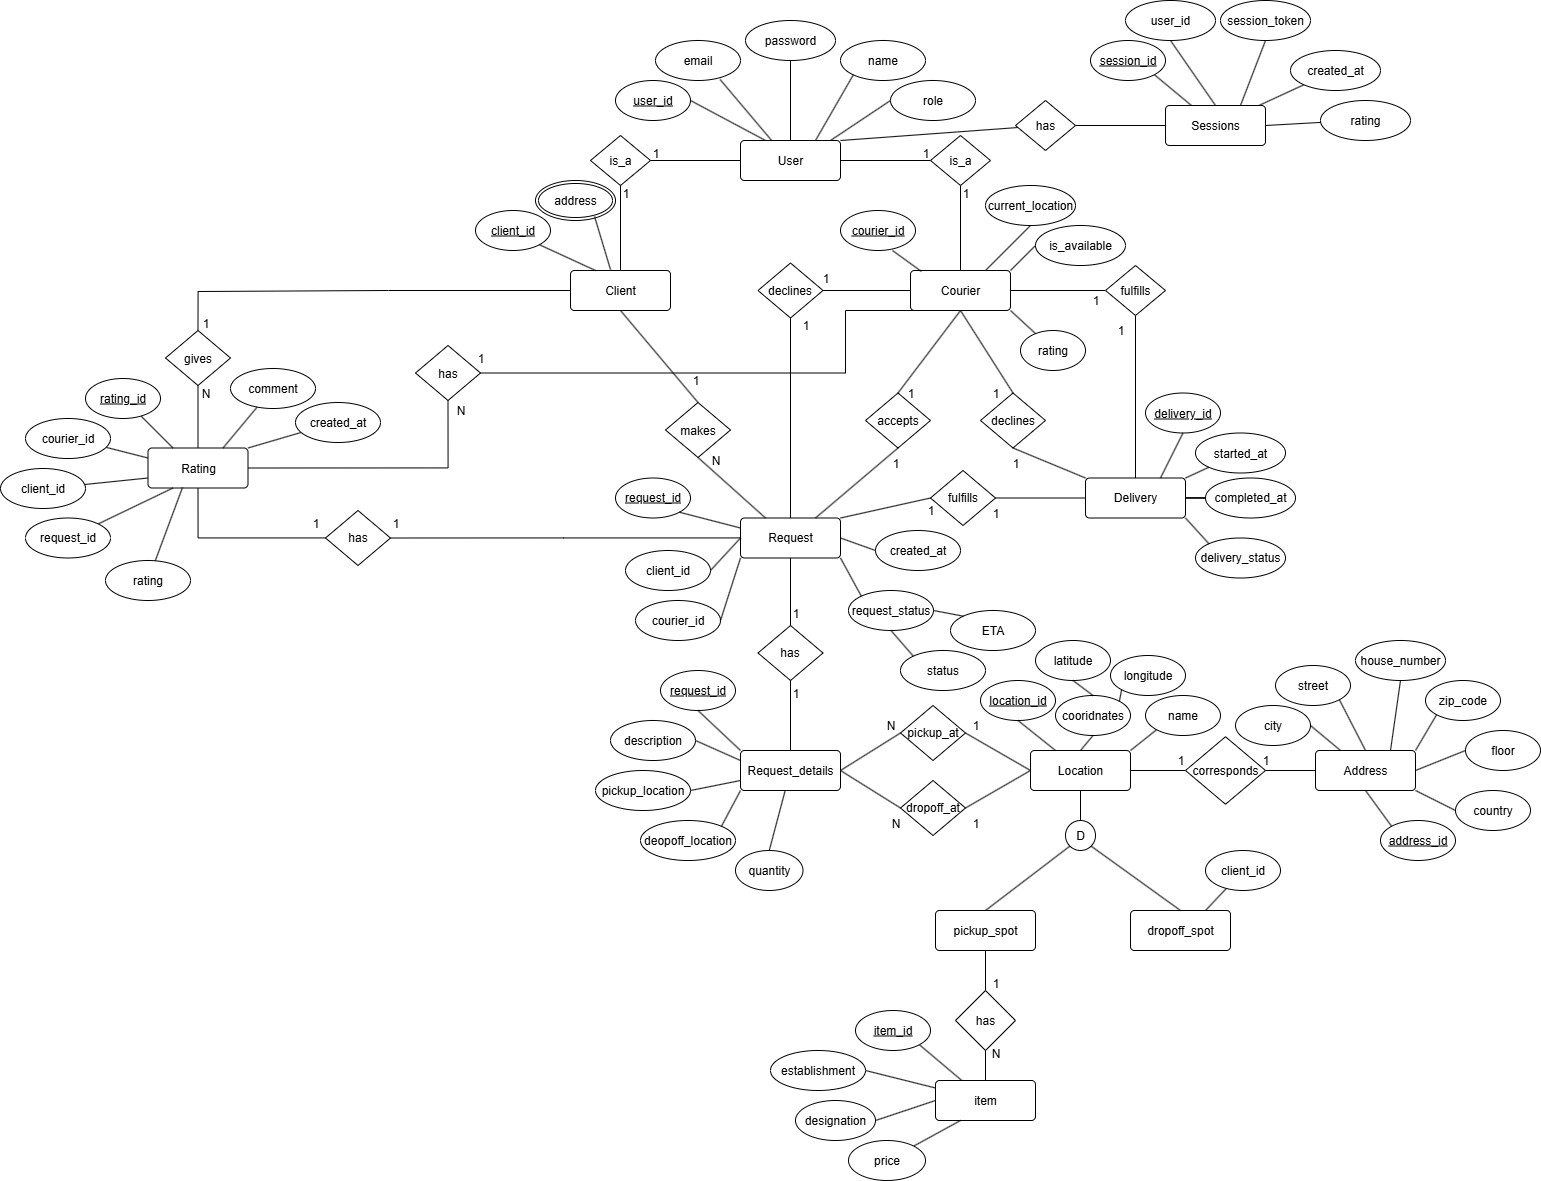
\includegraphics[angle=90, width=1.0\textwidth]{images/EA-model.png}
    \caption{EA model}
\end{figure}

\section{Entity Class Diagram}
\label{appendix:full-class-diagram}

This appendix provides the complete class diagram of the LiftDrop system. The diagram illustrates the main entities, their relationships, and the roles they play in the overall architecture.

\begin{figure}[H]
    \centering
    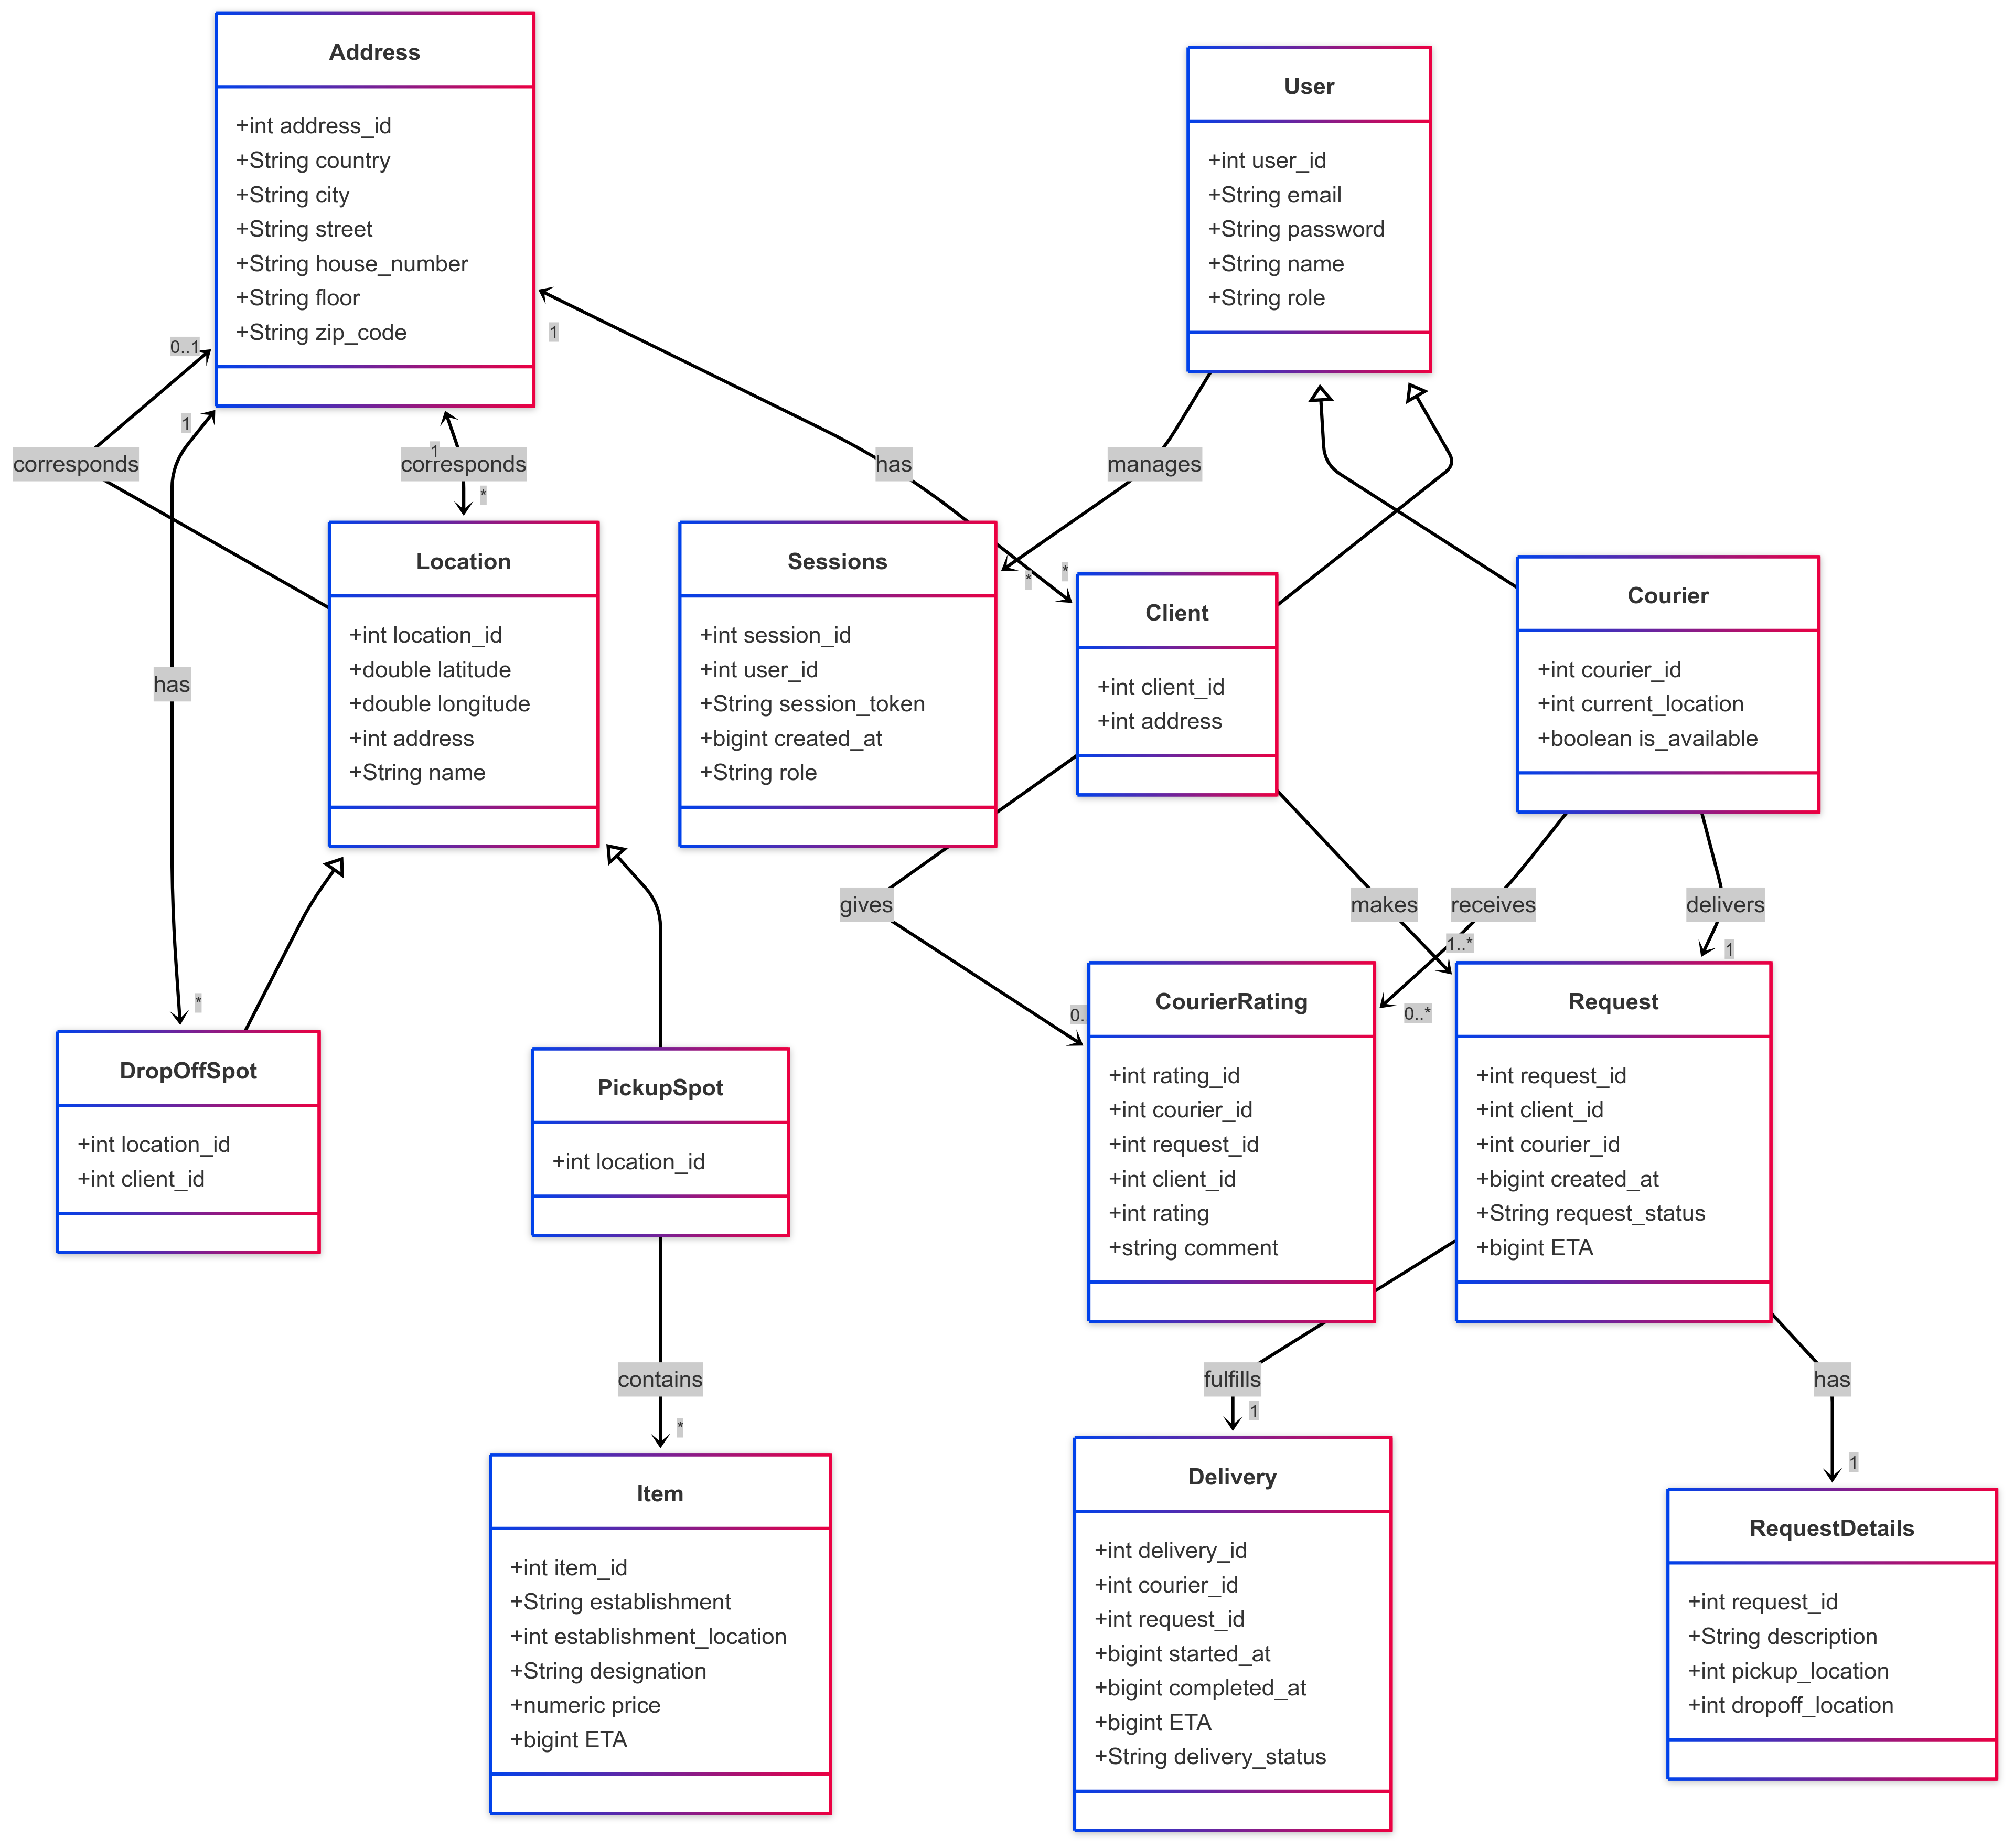
\includegraphics[width=0.95\textwidth]{images/classDiagrams/FullDiagram.png}
    \caption{Full Class Diagram of the LiftDrop System}
    \label{fig:class-diagram}
\end{figure}

\end{document}
